%% main.tex -- manuscript for the European Journal of Operational Research (EJOR)
%% Class: elsarticle, option `review' (single column, 1.5 line spacing, no line numbers), 11 pt.
%% References: biblatex-apa (APA 7th edition, as the EJOR Guide for Authors requires), compiled with biber.
%% Compile: latexmk -pdf main.tex   (or: pdflatex, biber, pdflatex, pdflatex)
\documentclass[review,11pt,nonatbib]{elsarticle}

\usepackage[a4paper,margin=2.5cm]{geometry}
\usepackage[T1]{fontenc}
\usepackage[british]{babel}
\usepackage{csquotes}
\usepackage{lmodern}
\usepackage{microtype}
\usepackage{amsmath,amssymb,amsthm}
\usepackage{booktabs}
\usepackage{tabularx}
\usepackage{array}
\usepackage{graphicx}
\usepackage{algorithm}
\usepackage{algpseudocode}
\usepackage[style=apa,backend=biber,doi=true,url=true]{biblatex}
\addbibresource{references.bib}
\usepackage{etoolbox}
\usepackage{xurl}
\usepackage[hidelinks,hypertexnames=false]{hyperref}
% The text is set at 1.5 line spacing (option `review'), as EJOR asks; tables and the algorithm are single-spaced.
\AtBeginEnvironment{table}{\linespread{1}\selectfont}
\AtBeginEnvironment{algorithm}{\linespread{1}\selectfont}

\journal{European Journal of Operational Research}

% ---------------------------------------------------------------- theorems
\newtheorem{proposition}{Proposition}
\newtheorem{lemma}{Lemma}
\theoremstyle{remark}
\newtheorem*{remark}{Remark}

% ---------------------------------------------------------------- notation
\newcommand{\tmin}{\tau_{\min}}
\newcommand{\tmax}{\tau_{\max}}
\newcommand{\Eref}{E_{\mathrm{ref}}}
\newcommand{\Ebar}{\bar{E}}
\newcommand{\Xin}{X^{\mathrm{in}}}
\newcommand{\Xout}{X^{\mathrm{out}}}
\newcommand{\inst}[1]{\texttt{\detokenize{#1}}}
\newcommand{\EUR}{\texteuro}
\newcommand{\CO}{CO\textsubscript{2}e}
\newcommand{\tr}[1]{\textsuperscript{#1}}
\renewcommand{\arraystretch}{1.12}
\newcolumntype{L}{>{\raggedright\arraybackslash}X}
\newcolumntype{R}[1]{>{\raggedleft\arraybackslash}p{#1}}

\begin{document}

\begin{frontmatter}

\title{Setting a carbon tax that anticipates the operator: a bilevel model for closed-loop supply chain network design}

%% TODO(author): complete the author list, affiliations, ORCID iDs and the corresponding e-mail address.
\author[uc]{Marcelo Pinto\corref{cor1}}
\ead{TODO@uc.pt}
\cortext[cor1]{Corresponding author.}
\author[uc]{TODO Co-author}
\affiliation[uc]{organization={TODO Department, University of Coimbra},
            addressline={TODO street address},
            postcode={TODO},
            city={Coimbra},
            country={Portugal}}

\begin{abstract}
A carbon tax reduces emissions only through the decisions it changes. We study how a regulator should set a carbon tax when the operator responds by redesigning a closed-loop supply chain. The regulator minimises the operator's emissions plus a small weight on the tax rate. The operator designs a multi-period, multi-product network, choosing suppliers, facilities, technologies and transport modes, and pays the tax on its discounted emissions. The result is a bilevel program with a continuous tax and a mixed-integer follower. We show that an optimal tax exists and lies where the operator switches to a cleaner network; a higher tax raises the tax bill by more than the further abatement is worth to the regulator. We solve the problem with a deterministic bounding procedure, adapted to a relaxation in which the tax multiplies a continuous emission aggregate, and state what each result certifies at the solver's tolerances. On 15 generated instances and a case study, the procedure closes the gap to 0.01\% on 11 of the 16 within one hour. On the nine closed instances whose optimal tax lies below 74 euros per tonne, the 2025 average European emission allowance price, a fixed tax at that price achieves the same reduction with a bill up to 73 times larger; on the other two it abates far less. The tax acts mostly through supplier choice in the generated instances and through cleaner technology and remanufacturing in the case study, and the cost of clean technology, more than the tax, sets how much is abated.
\end{abstract}

\begin{keyword}
OR in environment and climate change \sep Bilevel optimisation \sep Carbon tax \sep Closed-loop supply chain \sep Network design
\end{keyword}

\end{frontmatter}

% =====================================================================================
\section{Introduction}\label{sec:intro}

A regulator who anticipates how an operator redesigns its supply chain can choose the lowest carbon tax that induces the operator's cleanest response; a regulator who does not may overshoot or fall short. Carbon is priced in two ways: through cap-and-trade, where the market sets the price, as in the European Union Emissions Trading System, and through taxes, where the regulator does. In either case the price matters through the decisions it changes: which suppliers the operator buys from, which technologies and facilities it uses and how it moves goods \parencite{palak2014analyzing,marufuzzaman2014environmentally,drake2016technology,waltho2019green}.

In most studies of carbon pricing in supply chain planning and design, the price is a parameter, and the studies describe how the supply chain responds to it \parencite{fahimnia2015tactical,zakeri2015carbon,haddadsisakht2018closed,waltho2019green}. That response is not smooth. \textcite{zakeri2015carbon} observe an erratic, non-linear reduction in emissions, with inflection points, as the price rises, and \textcite{krass2013environmental} show that a firm's technology choice can even reverse as the tax rises. A regulator that wants to set the tax well must therefore anticipate how the supply chain will react, not merely observe it.

Choosing the tax is then a leader--follower problem, a bilevel program \parencite{kleinert2021survey}. The regulator sets the tax anticipating the operator's best response, and the operator designs its network given the tax. Existing bilevel models of environmental taxes either let the follower choose continuous quantities, so that it can be replaced by its optimality conditions \parencite{almutairi2014carbon}, or search over the policy on a grid \parencite{bard2000bilevel}, or solve integer followers by problem-specific branch-and-bound \parencite{liu2023optimal}. When the follower designs a closed-loop network with location, technology and fleet decisions, its problem is a mixed-integer linear program (MILP) whose objective contains the product of the tax and the emissions. General exact methods for mixed-integer bilevel programs either exclude this structure or do not exploit it. \textcite{fischetti2017new} exclude continuous leader variables from the lower level, and \textcite{lozano2017value} require the leader's variables to be integer. The bounding algorithm of \textcite{mitsos2008global} and the decomposition of \textcite{merkert2022exact} do admit products of leader and follower variables, but treat them in general, without using the fact that the tax leaves the operator's feasible set unchanged.

This paper sets a single carbon tax for an operator that designs a closed-loop supply chain (CLSC) with the multi-period, multi-product model of \textcite{mota2018sustainable}. The regulator minimises the operator's physical emissions plus a small weight on the tax rate, so that among taxes that abate the same, the lowest is chosen. We make four contributions.
\begin{enumerate}
\item A bilevel model in which a continuous carbon tax enters a mixed-integer CLSC design problem, with the operator taxed on its discounted emissions and the regulator counting physical ones. Using classical properties of parametric integer programs, we show that an optimal tax exists and lies at the lower end of the tax range or at a break point of the operator's value function (Proposition~\ref{prop:structure}).
\item An adaptation of the deterministic bounding procedure (DBP) of \textcite{soares2021deterministic} to a high-point relaxation in which the tax multiplies a continuous emission aggregate. It comes with valid bounds on that product, a statement of what each result certifies at the solver's tolerances (Proposition~\ref{prop:certificate}), and a discussion of when bounding is preferable to enumerating break points (Section~\ref{sec:enumeration}).
\item A computational study on 15 instances from the generator of \textcite{tautenhain2021efficient} and on the case study of \textcite{mota2018sustainable}, with a one-at-a-time sensitivity analysis of six parameters and a check of the results against tighter tolerances, other solver seeds and longer runs.
\item Policy findings, each stated with the instances that support it. The optimal tax lies at a break point; a fixed tax at the 2025 EU allowance price overshoots it on some instances and falls short on others; the mechanism of abatement depends on where the emissions arise; and the cost of clean technology, more than the tax, sets how much is abated.
\end{enumerate}

Section~\ref{sec:literature} reviews the literature. Section~\ref{sec:bilevel} recalls bilevel optimisation and characterises the problem's solutions. Section~\ref{sec:dbp} presents the DBP, its high-point relaxation and what each result certifies. Section~\ref{sec:model} states the model and the instances, Section~\ref{sec:results} reports the results, and Section~\ref{sec:conclusions} concludes.

\subsection{Related literature}\label{sec:literature}

Four streams meet in this paper: carbon pricing in supply chain planning and design, where the price is exogenous; closed-loop supply chains under emissions regulation; bilevel models of environmental policy and pricing, where the price is a decision; and exact methods for mixed-integer bilevel programs.

\paragraph{Carbon pricing in supply chain planning and design} Reviews of sustainable and green supply chain design \parencite{barbosapovoa2018opportunities,waltho2019green} find that carbon caps, offsets, cap-and-trade and taxes all achieve substantial reductions at a slight increase in cost, mostly by moving the supply chain to lower-emitting resources \parencite{waltho2019green}. \textcite{chaabane2012design} design supply chains with life-cycle emissions under emissions trading. \textcite{palak2014analyzing} and \textcite{marufuzzaman2014environmentally} show how cap, tax, cap-and-trade and offset mechanisms change supplier, transport-mode and facility decisions. \textcite{fahimnia2015tactical} ask which carbon price gives the best environmental return per unit of added supply chain cost, and \textcite{drake2016technology} compare a tax with cap-and-trade in the choice of technology and capacity. \textcite{mota2018sustainable} integrate facility location and capacity, supplier selection, technology choice, intermodal transport and remanufacturing in one model, which \textcite{tautenhain2021efficient} solve with a Lagrangian matheuristic on generated instances. In all of these the price of carbon is a parameter.

\paragraph{Closed-loop supply chains under emissions regulation} Closed-loop supply chain research has grown from a technical niche into a subfield of supply chain management \parencite{guide2009or,govindan2015reverse}. Network design models range from generic reverse logistics MILPs \parencite{salema2007optimization} to stochastic designs under demand and return uncertainty \parencite{uster2017closed} and designs under a carbon tax \parencite{haddadsisakht2018closed,govindan2023location}. Game-theoretic studies ask how emissions taxes interact with remanufacturing: \textcite{savaskan2004closed} model reverse channels led by a Stackelberg manufacturer, and \textcite{yenipazarli2016managing} characterises the taxes under which remanufacturing lowers emissions and raises profit.

\paragraph{Bilevel models of environmental policy and pricing} \textcite{labbe1998bilevel} formulate the bilevel taxation problem, in which a leader sets taxes on a network and the follower reacts, and show that it is NP-complete in general; \textcite{marcotte2009toll} use tolls to steer the routes of hazardous-materials carriers. \textcite{amouzegar1999determining} let a government set taxes that steer the location and capacity of waste treatment facilities. \textcite{bard2000bilevel} set biofuel tax credits for a farm sector modelled as a linear program, searching over a grid of credits. \textcite{almutairi2014carbon} set a carbon tax on an industry's emission factor and replace the continuous follower by its optimality conditions. \textcite{krass2013environmental} and \textcite{rustico2022environmental} analyse regulators who set taxes to induce green technology, and \textcite{liu2023optimal} solve a bilevel integer program with a government leader by branch-and-bound. \textcite{caselli2026bilevel} survey bilevel models with a sustainability perspective, many of them pricing problems.

\paragraph{Exact methods for mixed-integer bilevel programs} When the follower has integer variables, its optimality cannot be expressed by optimality conditions, and the relaxation obtained by dropping it is weak \parencite{moore1990mixed}. Exact methods work instead with the follower's optimal value function \parencite{kleinert2021survey}. They include branch-and-cut \parencite{fischetti2017new,tahernejad2020branch}, value-function reformulations \parencite{lozano2017value,tavasloglu2019solving}, projection and decomposition \parencite{yue2019projection,merkert2022exact}, multi-parametric programming \parencite{avraamidou2019multi}, and bounding procedures that alternate a relaxation with the follower's response \parencite{mitsos2008global}. \textcite{soares2021deterministic} propose the DBP for a retailer that sets time-of-use tariffs while consumers schedule their appliances. \textcite{soares2020designing} estimate bounds when the consumers' problem cannot be solved exactly, and \textcite{soares2023deterministic} apply a deterministic bounding algorithm to a mixed-integer nonlinear version. In these pricing problems the prices multiply binary follower variables, so the high-point relaxation is a MILP. \textcite{merkert2022exact} solve problems with products of leader and follower variables exactly in general.

\begin{table}[!htbp]
\centering
\caption{Bilevel models in which a public or pricing leader steers a follower, and this paper.}\label{tab:positioning}
\footnotesize
\begin{tabularx}{\textwidth}{@{}>{\raggedright\arraybackslash}p{2.35cm}LLLLL@{}}
\toprule
Study & Leader's decision & Follower's problem & How the leader's decision enters the follower & Method & Guarantee \\
\midrule
\textcite{bard2000bilevel} & Biofuel tax credits & Crop and set-aside choice of a farm sector (linear program) & Crop prices & Grid search over the credits; approximate nonlinear program & Up to the grid \\
\textcite{krass2013environmental} & Tax, subsidy and rebate & Technology, quantity and price of a monopolist & Costs & Analytical & Closed form, stylised model \\
\textcite{almutairi2014carbon} & Tax on the emission factor & Output of an industry (continuous) & Costs & Optimality conditions, then a MILP & Exact for a continuous follower \\
\textcite{soares2021deterministic} & Time-of-use prices & Appliance scheduling (MILP) & Prices times binary variables & DBP with a MILP relaxation & Bounds; optimal to tolerances \\
\textcite{merkert2022exact} & General & Mixed-integer, with nonlinear terms & Products of leader and follower variables & Projection-based decomposition & Exact under an assumption \\
\textcite{liu2023optimal} & Subsidy & Trauma care network redesign (integer) & Subsidy & Branch-and-bound & Exact \\
This paper & Carbon tax & Multi-period CLSC network design (MILP) & Tax times a continuous emission aggregate & DBP with a bilinear relaxation & Bounds; optimal to stated tolerances (Proposition~\ref{prop:certificate}) \\
\bottomrule
\end{tabularx}
\end{table}

This paper takes the operator's problem from the first two streams, the leader--follower view from the third and the method from the fourth. It differs from the bilevel tax models in its follower, a full CLSC design problem, and in solving the problem with bounds. It differs from \textcite{soares2021deterministic,soares2023deterministic} in that the tax multiplies a continuous emission aggregate, so the high-point relaxation is bilinear in two continuous quantities.

% =====================================================================================
\section{Bilevel optimisation}\label{sec:bilevel}

A bilevel problem couples two optimisation problems in a hierarchy: the leader decides first, anticipating the follower's response, and the follower then optimises its own objective over a feasible set that may depend on the leader's decision. With both levels minimising, the general problem reads
\begin{equation*}
\text{``}\min_{x \in X}\text{''} \; F(x, y) \quad \text{s.t.} \quad G(x, y) \le 0, \quad y \in \arg\min_{y' \in Y} \bigl\{ f(x, y') : g(x, y') \le 0 \bigr\},
\end{equation*}
where $x$ and $y$ are the leader's and the follower's decisions, $X$ and $Y$ may impose integrality, $F$ and $f$ are their objectives and $G$ and $g$ their constraints. For a leader's decision $x$, the follower's feasible set is $Y(x) = \{y \in Y : g(x, y) \le 0\}$ and its rational reaction set is $\Psi(x) = \arg\min \{f(x, y) : y \in Y(x)\}$. The induced region $\{(x, y) : x \in X,\ G(x, y) \le 0,\ y \in \Psi(x)\}$ is the feasible set of the bilevel problem. Even linear bilevel problems are hard: their value questions climb the polynomial hierarchy \parencite{jeroslow1985polynomial}, and the bilevel taxation problem is NP-complete \parencite{labbe1998bilevel}. When the leader's variables are continuous and the follower's discrete, the induced region need not be closed, and an optimal solution may fail to exist \parencite{soares2021deterministic}.

The quotation marks express an ambiguity: when $\Psi(x)$ has several elements, $F$ depends on which one the follower chooses. The optimistic convention assumes that the follower chooses, among its optimal responses, the one best for the leader; the pessimistic convention assumes the worst. We adopt the optimistic convention, as \textcite{soares2021deterministic} do, so the problem becomes the minimisation of $F$ over $x$ and $y$ jointly, subject to $y \in \Psi(x)$. In computation the follower's optimality holds only to a tolerance. With $\varepsilon' > 0$, the $\varepsilon'$-optimistic problem lets the follower choose any response within $\varepsilon'$ of its optimum, as in the bounding algorithms of \textcite{mitsos2008global}, which terminate at points that are $\varepsilon$-optimal in both the inner and the outer program.

The DBP addresses problems in which the leader's constraints do not involve the follower's variables and the follower's constraints do not involve the leader's: $G(x, y) = G(x)$ and $g(x, y) = g(y)$. Pricing problems belong to this class, and so does ours. The leader's decision is a single continuous tax rate $x = \tau \in [\tmin, \tmax]$. The follower's feasible set $Y$, given by the network design constraints of Section~\ref{sec:model}, does not depend on $\tau$. The tax enters only the follower's objective, $f(\tau, y) = c(y) + \tau\,\beta(y)/1000$, where $c(y)$ is the operator's cost in \EUR\ and $\beta(y)$ its discounted emissions in kg; the leader minimises $F(\tau, y) = E(y) + \mu\,\tau$, with $E(y)$ the physical emissions and $\mu > 0$ a weight. The following result collects properties of the follower's value function that are classical in parametric integer programming \parencite{geoffrion1977parametric,jenkins1982parametric} and draws their consequences for the leader: existence, and a finite set of candidate taxes.

\begin{proposition}\label{prop:structure}
Let $Y$ be nonempty and bounded, with integer variables taking finitely many values, and let $c$, $\beta$ and $E$ be linear in $y$. Let $\phi(\tau) = \min \{f(\tau, y) : y \in Y\}$, let $\Psi(\tau)$ be its set of minimisers, and let $E^\circ(\tau) = \min \{E(y) : y \in \Psi(\tau)\}$ be the emissions of the optimistic response.
\begin{enumerate}
\item[(a)] $\phi$ is concave, continuous and piecewise linear on $[\tmin, \tmax]$, with finitely many break points $b_1 < \dots < b_m$ in $(\tmin, \tmax)$.
\item[(b)] On each open interval between consecutive points of $\{\tmin, b_1, \dots, b_m, \tmax\}$, $\Psi(\tau)$ and $E^\circ(\tau)$ are constant. At each end of such an interval, $\Psi$ contains the interval's set, so $E^\circ$ at a break point is at most its value on either adjacent interval.
\item[(c)] The optimistic problem $\min \{E^\circ(\tau) + \mu\,\tau : \tau \in [\tmin, \tmax]\}$ has an optimal solution, and every optimal tax lies in $\{\tmin, b_1, \dots, b_m\}$.
\item[(d)] For $\varepsilon' > 0$, the $\varepsilon'$-optimistic problem $\min \{E(y) + \mu\,\tau : \tau \in [\tmin, \tmax],\ y \in Y,\ f(\tau, y) \le \phi(\tau) + \varepsilon'\}$ has an optimal solution.
\end{enumerate}
\end{proposition}

\begin{proof}
(a) Fixing the integer variables at one of their finitely many values leaves a bounded polyhedron, on which a linear function attains its minimum at one of finitely many vertices. Hence $\phi$ is the minimum of finitely many affine functions $\tau \mapsto c(v) + \tau\,\beta(v)/1000$, one per vertex $v$, which proves (a). (b) Let $J$ be such an interval, on which $\phi$ is affine, and let $y \in \Psi(\tau_0)$ for some $\tau_0$ in $J$. The affine function $\tau \mapsto f(\tau, y)$ lies above $\phi$ and touches it at the interior point $\tau_0$, so it coincides with $\phi$ on $J$ and, by continuity, at both ends of $J$. Hence $y \in \Psi(\tau)$ for every $\tau$ in the closure of $J$. Each $\Psi(\tau)$ is a finite union of faces of bounded polyhedra, so the minimum that defines $E^\circ$ is attained. (c) On $J$ the leader's objective equals $E^\circ(J) + \mu\,\tau$. Since $\mu > 0$, it exceeds its value at the left end $a$ of $J$, where $E^\circ(a) \le E^\circ(J)$ by (b). The minimum over $[\tmin, \tmax]$ is therefore the least of finitely many values, taken at $\tmin$ or at a break point. (d) Since $f$ and $\phi$ are continuous and $Y$ is closed and bounded, the feasible set is nonempty and compact, and the objective is continuous.
\end{proof}

Two remarks follow. First, responses in $\Psi(\tau)$ share the cost and the tax base but can differ in $E$, because $\beta$ discounts emissions and $E$ does not; the optimistic tie-break is therefore needed even between break points. Second, under the pessimistic convention $E$ at a break point would take the larger of the adjacent values, and the infimum would in general not be attained. Proposition~\ref{prop:structure}(c) reduces the leader's choice to finitely many candidates; Section~\ref{sec:enumeration} discusses what this implies for the choice of method.

The break points are the operator's \emph{switching prices}: the taxes at which it moves from one network to another. Their level depends on how emission-intensive the operator is, in a simple way.

\begin{proposition}\label{prop:scale}
Let every emission factor be multiplied by $k > 0$, so that $E$ and $\beta$ become $kE$ and $k\beta$ while $c$ is unchanged, and let $\phi_k$, $\Psi_k$ be the follower's value function and response set after scaling. Then
\begin{enumerate}
\item[(a)] $\Psi_k(\tau) = \Psi(k\tau)$ and $\phi_k(\tau) = \phi(k\tau)$, so every break point is divided by $k$;
\item[(b)] at $\tau$ after scaling and at $k\tau$ before, each response has the same cost and the same tax bill, $\tau\,k\beta(y)/1000$, so the tax bill as a share of the operator's cost is the same;
\item[(c)] with $\mu = \xi\,\Eref$, the regulator's problem after scaling is the problem before scaling with the weight $\xi/k$ on the range $[k\tmin, k\tmax]$, its optimal tax divided by $k$.
\end{enumerate}
\end{proposition}
\begin{proof}
(a) and (b): $c(y) + \tau\,k\beta(y)/1000 = f(k\tau, y)$ for every $y \in Y$. (c) $\Eref$ scales by $k$, hence so does $\mu$, and $kE(y) + k\mu\,\tau = k\,[E(y) + (\mu/k)\,(k\tau)]$; substituting $\tau' = k\tau$ gives the problem before scaling with weight $\mu/k$ over $\tau' \in [k\tmin, k\tmax]$.
\end{proof}

Proposition~\ref{prop:scale} separates what a tax level means from the data that set it. A switching price found on an operator that emits $\iota$ kg \CO\ per euro of cost corresponds to a tax $\iota/\iota'$ times higher on an otherwise identical operator that emits $\iota'$, at the same tax bill relative to cost. We use the bill share, $\tau\,\beta(y)/(1000\,c(y))$, to compare switching prices across instances and with an observed carbon price (Section~\ref{sec:anticipation}).

% =====================================================================================
\section{The deterministic bounding procedure}\label{sec:dbp}

\subsection{Foundations}\label{sec:foundations}

The DBP of \textcite{soares2021deterministic} generates lower and upper bounds on the leader's optimal value until they meet. Like the bounding algorithms of \textcite{mitsos2008global} and \textcite{mitsos2010global}, it alternates a relaxation, tightened by cuts on the follower's value function, with the follower's response at the relaxation's proposal. Their leader maximises and ours minimises, so the roles of the bounds are swapped: here the relaxation gives the lower bound and the follower's response the upper bound. The optimistic bilevel problem is
\begin{equation}
\min_{\tau,\, y} \; F(\tau, y) = E(y) + \mu\,\tau \quad \text{s.t.} \quad \tmin \le \tau \le \tmax, \quad y \in \arg\min_{y' \in Y} f(\tau, y'), \tag{P1}\label{P1}
\end{equation}
with $f(\tau, y) = c(y) + \tau\,\beta(y)/1000$. Dropping the follower's optimality gives the high-point relaxation (HPR)
\begin{equation}
\min_{\tau,\, y} \; F(\tau, y) \quad \text{s.t.} \quad \tmin \le \tau \le \tmax, \quad y \in Y, \tag{P2}\label{P2}
\end{equation}
whose optimal value is a lower bound LB on that of \eqref{P1}. For a tax $\tau_k$, the follower's problem
\begin{equation}
f^*_k = \min_{y \in Y} f(\tau_k, y) \tag{P3}\label{P3}
\end{equation}
gives its optimal value, and its optimistic response solves
\begin{equation}
\min_{y \in Y} \; E(y) \quad \text{s.t.} \quad f(\tau_k, y) \le f^*_k + \varepsilon' \, |f^*_k|. \tag{P4}\label{P4}
\end{equation}

\begin{lemma}\label{lem:ub}
Let $y_k$ solve \eqref{P4} with $\varepsilon' = 0$. Then $(\tau_k, y_k)$ is feasible for \eqref{P1}, and $F(\tau_k, y_k)$ is an upper bound UB on its optimal value.
\end{lemma}
\begin{proof}
The constraint of \eqref{P4} makes $y_k$ optimal for \eqref{P3}; its objective selects, among the follower's optimal responses, the one with the least emissions, which minimises $F$ at $\tau_k$.
\end{proof}

A small tolerance $\varepsilon' > 0$, relative to the follower's objective, avoids losing feasibility to floating-point arithmetic, as in \textcite{soares2021deterministic} and \textcite{mitsos2010global}; the problem solved is then the $\varepsilon'$-optimistic one of Section~\ref{sec:bilevel}. Given the responses $y_1, \dots, y_K$ obtained so far, the HPR with value-function cuts is
\begin{equation}
\begin{aligned}
\min_{\tau,\, y} \; & F(\tau, y) \\
\text{s.t.} \; & \tmin \le \tau \le \tmax, \quad y \in Y, \quad f(\tau, y) \le f(\tau, y_k), \; k = 1, \dots, K.
\end{aligned} \tag{P5}\label{P5}
\end{equation}

\begin{lemma}\label{lem:lb}
The optimal value of \eqref{P5} is a lower bound on that of \eqref{P1}.
\end{lemma}
\begin{proof}
$Y$ does not depend on $\tau$, so every $y_k$ is feasible for the follower at every tax. For any $\tau$, the follower's optimal value is therefore at most $f(\tau, y_k)$, and every optimal response satisfies the cuts. No feasible point of \eqref{P1} is removed, and \eqref{P5} is a relaxation of \eqref{P1}.
\end{proof}

\begin{lemma}\label{lem:stop}
Let $\tau_{K+1}$ be the tax of an optimal solution $(\tau_{K+1}, y')$ of \eqref{P5} with $K$ cuts, and let every subproblem be solved exactly with $\varepsilon' = 0$. If $\tau_{K+1} = \tau_K$, an optimal solution of \eqref{P1} has been found.
\end{lemma}
\begin{proof}
\eqref{P5} contains $f(\tau, y) \le f(\tau, y_K)$, so at $\tau_K$ the point $y'$ is optimal for the follower. Its value $F(\tau_K, y')$ is the optimum of a relaxation, hence at most the optimum of \eqref{P1}, and at least $F(\tau_K, y_K)$ by the choice of $y_K$ in \eqref{P4}. The bounds coincide.
\end{proof}

Unlike \textcite{soares2021deterministic}, we add no $\varepsilon'$ to the right-hand side of the cuts. The response $y_k$ already lies up to $\varepsilon'$ above the follower's optimum, and a second tolerance in the cut would let \eqref{P5} propose a tax at which a lower-emission response lies outside the tie-break set of \eqref{P4}; the follower would never return it, and the procedure would stall. Since the tax is continuous, \eqref{P5} returns $\tau_K$ again only up to the solver's tolerances; we apply the test of Lemma~\ref{lem:stop} when $|\tau_{K+1} - \tau_K| \le \delta_\tau = 0.001$~\EUR/t.

\begin{lemma}\label{lem:finite}
Let every subproblem be solved exactly with $\varepsilon' = 0$, and let \eqref{P4} return an extreme point of its feasible set. Then the bounds meet after finitely many iterations.
\end{lemma}
\begin{proof}
For a fixed value of the integer variables, the feasible set of \eqref{P4} is empty or a face of a bounded polyhedron, so its extreme points are vertices of that polyhedron; the responses therefore belong to a finite set. Suppose the response $y_{K+1}$ at $\tau_{K+1}$ equals an earlier response $y_j$, $j \le K$. The point $(\tau_{K+1}, y')$ proposed by \eqref{P5} satisfies $f(\tau_{K+1}, y') \le f(\tau_{K+1}, y_j) = \phi(\tau_{K+1})$, so $y'$ is optimal for the follower at $\tau_{K+1}$, and $E(y') \ge E(y_{K+1})$ by \eqref{P4}. Hence $\mathrm{LB} \ge F(\tau_{K+1}, y') \ge F(\tau_{K+1}, y_{K+1}) \ge \mathrm{UB}$, and the bounds meet. A new response appears at every iteration until then, which can happen only finitely often.
\end{proof}

Lemmas~\ref{lem:ub} and~\ref{lem:stop} assume exact solves, whereas every subproblem is solved to a relative mixed-integer programming (MIP) gap. The next result states what the bounds certify at the tolerances actually used.

\begin{proposition}\label{prop:certificate}
Suppose each solve of \eqref{P3} at $\tau_k$ returns a value $\bar f_k$ with relative MIP gap at most $\bar g$, so that $\phi(\tau_k) \ge \bar f_k - \bar g\,|\bar f_k|$, and that its tie-break response satisfies $f(\tau_k, y_k) \le \bar f_k + \varepsilon'\,|\bar f_k|$. Let LB be a dual bound of \eqref{P5}, let $\mathrm{UB} = F(\hat\tau, \hat y)$ be the least value evaluated, attained by the incumbent $(\hat\tau, \hat y)$, and let $v^*$ be the optimal value of \eqref{P1}. Then
\begin{enumerate}
\item[(i)] $\mathrm{LB} \le v^*$;
\item[(ii)] $f(\hat\tau, \hat y) \le \phi(\hat\tau) + (\bar g + \varepsilon')\,|\bar f|$, where $\bar f$ is the follower's value at $\hat\tau$; and
\item[(iii)] if $(\mathrm{UB} - \mathrm{LB})/\max(1, |\mathrm{UB}|) \le \varepsilon$, then $F(\hat\tau, \hat y) \le v^* + \varepsilon \max(1, |\mathrm{UB}|)$.
\end{enumerate}
\end{proposition}
\begin{proof}
(i) The proof of Lemma~\ref{lem:lb} uses only $y_k \in Y$, so \eqref{P5} relaxes \eqref{P1} whatever the quality of the responses $y_k$; a dual bound of \eqref{P5} is at most its optimal value, hence at most $v^*$. (ii) Combine the two assumptions at $\hat\tau$. (iii) $\mathrm{UB} \le \mathrm{LB} + \varepsilon \max(1, |\mathrm{UB}|) \le v^* + \varepsilon \max(1, |\mathrm{UB}|)$ by (i).
\end{proof}

The incumbent is thus a response that is optimal for the operator to within the MIP gap plus $\varepsilon'$, and whose leader value exceeds the exact optimistic optimum by at most $\varepsilon$ in relative terms. This is what ``optimal to stated tolerances'' means in this paper. The two bounds refer to slightly different problems: LB to the exact one, UB to a nearly optimal response. The gap can therefore be negative by a round-off amount, as on \inst{STD_I25_M4_T12} (Table~\ref{tab:main}). With $\bar g = \varepsilon = 10^{-4}$ (Section~\ref{sec:results}), the final gap may coincide with the HPR's own MIP gap.

Proposition~\ref{prop:certificate} bounds $F$, not $\tau$. Two taxes on the same plateau of $E^\circ$ differ in $F$ by $\mu\,|\Delta\tau|$, so the stopping test cannot separate taxes closer than $\varepsilon \max(1, |\mathrm{UB}|)/\mu$. With $\mu = \xi\,\Eref$ (Section~\ref{sec:model}) and UB close to $\Eref$, this resolution is about $\varepsilon/\xi$, which is \EUR1/t for the settings of Section~\ref{sec:results}. The reported taxes are more stable than this worst case. When the MIP gap is tightened to $10^{-6}$, 51 of 52 small-instance runs return the same tax to within \EUR0.05/t, and with five solver seeds 19 of 20 runs return the same tax (Section~\ref{sec:robustness}).

\subsection{The algorithm}\label{sec:algorithm}

The procedure follows the steps of \textcite[Section~3.2]{soares2021deterministic}, with the lower and upper bounds exchanged for a minimising leader (Algorithm~\ref{alg:dbp}). Step~1 first solves \eqref{P2} without the term $\mu\,\tau$; its dual bound $\Eref$ is a lower bound on the emissions of any network and sets $\mu = \xi\,\Eref$. When the gap closes, the incumbent satisfies Proposition~\ref{prop:certificate}(iii); it is classed as optimal if, in addition, $|\tau_{k+1} - \tau_k| \le \delta_\tau$ and no subproblem behind the bounds stopped on its time limit (Lemma~\ref{lem:stop}), and as $\varepsilon$-optimal if not.

\begin{algorithm}[!htbp]
\caption{The DBP of \textcite{soares2021deterministic} as implemented here, for a minimising leader.}\label{alg:dbp}
\begin{algorithmic}[1]
\Require tolerances $\varepsilon$, $\varepsilon'$, $\delta_\tau$; relative weight $\xi$; stagnation limit $s_{\max} = 10$; run budget
\State Solve \eqref{P2} without $\mu\,\tau$; set $\Eref \gets$ its dual bound and $\mu \gets \xi\,\Eref$
\State Solve \eqref{P2}; set LB $\gets$ its dual bound, $\tau_1 \gets$ its tax, UB $\gets +\infty$, $k \gets 1$
\Loop
  \State Solve \eqref{P3} at $\tau_k$ to obtain $f^*_k$ \Comment{follower}
  \State Solve \eqref{P4} at $\tau_k$ to obtain $y_k$ \Comment{optimistic response}
  \If{$F(\tau_k, y_k) < \mathrm{UB}$}
     \State UB $\gets F(\tau_k, y_k)$; incumbent $\gets (\tau_k, y_k)$ \Comment{ties keep the lower tax}
  \EndIf
  \State Add the cut $f(\tau, y) \le f(\tau, y_k)$ to \eqref{P5} and solve it
  \State $\tau_{k+1} \gets$ its tax; LB $\gets \max(\mathrm{LB}, \text{its dual bound})$
  \If{$(\mathrm{UB} - \mathrm{LB})/\max(1, |\mathrm{UB}|) \le \varepsilon$}
     \If{$|\tau_{k+1} - \tau_k| \le \delta_\tau$ and no subproblem stopped on its time limit}
        \State \Return incumbent, classed \emph{optimal}
     \Else
        \State \Return incumbent, classed \emph{$\varepsilon$-optimal}
     \EndIf
  \EndIf
  \If{neither bound has moved for $s_{\max}$ iterations, or the budget is spent}
     \State \Return incumbent and [LB, UB], classed \emph{bounds}
  \EndIf
  \State $k \gets k + 1$
\EndLoop
\end{algorithmic}
\end{algorithm}

Each iteration solves one follower problem in two stages and one relaxation. The relaxation only gains constraints, so its optimum can only rise; its dual bound, read at a MIP gap, can fluctuate within that gap, so LB is kept monotone by taking the maximum over iterations.

\subsection{The bilinear high-point relaxation}\label{sec:hpr}

The HPR is where our problem departs from that of \textcite{soares2021deterministic}. Their prices multiply binary variables, and the product is linearised exactly. Here the tax multiplies the continuous aggregate $\beta(y)$, so the HPR contains the bilinear term $\tau\,\beta(y)$. We keep it as a single non-convex equality, $p = \tau\,\beta$, shared by all cuts, and solve the HPR by the spatial branch-and-bound of Gurobi 13.0.1; branch-and-cut over polyhedral relaxations of this kind is standard in global optimisation \parencite{tawarmalani2005polyhedral}. The solver relaxes $p$ by the envelopes of \textcite{mccormick1976computability}, which are exact only at the corners of the box of the operands, so we keep that box as narrow as the run allows:
\begin{equation*}
E(y) \ge \Eref, \qquad d_{\min}\, \Eref \le \beta(y) \le d_{\max}\, \Ebar, \qquad \tmin\, \beta_{\min} \le p \le \tmax\, \beta_{\max}.
\end{equation*}
Here $\Eref$ is the dual bound of the HPR solved without cuts and without the term $\mu\,\tau$, $\Ebar$ bounds the emissions with every facility and technology at capacity, $d_{\min}$ and $d_{\max}$ are the smallest and largest discount factors, and $\beta_{\min}$ and $\beta_{\max}$ are the bounds on $\beta$. None of these bounds removes a point of the HPR. The lower bound on $\beta$ matters. With $\tmin = 0$ and $\beta_{\min} = 0$, the first lower McCormick inequality reduces to $p \ge 0$, whereas $\beta_{\min} > 0$ turns it into $p \ge \beta_{\min}\,\tau$.

Relaxations that discretise one operand of the product would give a MILP instead of spatial branching. Options include piecewise McCormick envelopes with tightened bounds \parencite{castro2015tightening}, the multiparametric disaggregation technique, which scales better than piecewise McCormick envelopes on bilinear programs \parencite{kolodziej2013global}, and binary expansion of an integer operand \parencite{gupte2013solving}. \textcite{soares2023deterministic} handle a nonlinear follower within the same bounding scheme. We keep the solver's spatial branch-and-bound, which leaves the HPR exact. Section~\ref{sec:performance} shows that the HPR dominates the computing time, which makes these relaxations the first candidates for speeding up the method.

\subsection{Subproblems that stop with a MIP gap}\label{sec:gaps}

On the larger instances, subproblems reach their time limit before their MIP gap target. We follow the remedies of \textcite[Section~7]{soares2021deterministic}, which build on their bound estimates for followers that cannot be solved exactly \parencite{soares2020designing}, so that every bound reported remains a bound.

\paragraph{Lower bound} LB is the HPR's proven dual bound, not the value of its incumbent, so it remains valid whatever the HPR's gap. \textcite{soares2021deterministic} estimate the corresponding bound as the incumbent's value corrected by the MIP gap; the dual bound gives the same guarantee directly. An HPR that stops on its time limit with a point still proposes its tax.

\paragraph{Follower with a gap} If \eqref{P3} stops on its time limit with value $\bar f$ and relative gap $g$, the subproblem
\begin{equation}
\min_{y \in Y,\, \zeta \ge 0} \; \zeta \quad \text{s.t.} \quad f(\tau_k, y) \le \bar f\,(1 - g) + \zeta \tag{P6}\label{P6}
\end{equation}
searches for a better response, started from the incumbent of \eqref{P3}; $\bar f(1 - g)$ is the solver's bound on the follower's optimum, so a response with $\zeta$ close to zero is nearly optimal. Its response replaces that of \eqref{P3} if it improves $f$. If \eqref{P4} then finds no point within its budget, the response of \eqref{P3} or \eqref{P6} is kept. Such a response is not proven optimal, so the UB it gives is reported as not certified, and the result can be $\varepsilon$-optimal at best.

\paragraph{Relaxation without a point} The first time \eqref{P5} returns no point within its budget, its cuts are made elastic, as in (P5-D) of \textcite{soares2021deterministic}:
\begin{equation}
\begin{aligned}
\min_{\tau,\, y,\, \zeta} \; & F(\tau, y) + \Lambda \sum_{k} \zeta_k \\
\text{s.t.} \; & \tmin \le \tau \le \tmax, \; y \in Y, \; f(\tau, y) \le f(\tau, y_k) + \zeta_k, \; \zeta_k \ge 0, \; k = 1, \dots, K.
\end{aligned} \tag{P5-D}\label{P5D}
\end{equation}
The penalty $\Lambda$ exceeds the whole range of $F$, so a positive $\zeta_k$ is chosen only where no point satisfies every cut within the solver's reach; it never weakens the lower bound, because points with $\zeta = 0$ keep their value. A result whose last relaxation has an active slack cannot be classified as optimal.

\paragraph{Stopping} Because elastic variables and gaps can prevent convergence, the procedure also stops after 10 consecutive iterations in which neither bound changes \parencite{soares2021deterministic}, or when a run budget is spent; the budget is checked between subproblems and caps each subproblem's time limit.

\subsection{What a result certifies}\label{sec:classes}

Every result reports both bounds and the incumbent and is assigned one of four classes (Table~\ref{tab:classes}). The first two classes certify Proposition~\ref{prop:certificate}(iii); they differ only in the test of Lemma~\ref{lem:stop}, which asks whether the HPR has any other tax to propose at the tolerances used.

\begin{table}[!htbp]
\centering
\caption{Result classes. All conditions hold up to the solver's tolerances and $\varepsilon'$. The classes certify the leader's value; the tax itself is determined only to the resolution $\varepsilon \max(1, |\mathrm{UB}|)/\mu$ of Section~\ref{sec:foundations}, whatever the class.}\label{tab:classes}
\small
\begin{tabularx}{\textwidth}{@{}lL@{}}
\toprule
Class & Condition \\
\midrule
Optimal & Gap at most $\varepsilon$; the HPR re-proposes the evaluated tax within $\delta_\tau = 0.001$~\EUR/t; no subproblem behind the bounds stopped on its time limit; no elastic slack of \eqref{P5D} is active \\
$\varepsilon$-optimal & Gap at most $\varepsilon$, but one of the other conditions fails \\
Bounds & The run ended before the gap closed (budget, iteration cap or stagnation); the result is the interval [LB, UB] and the incumbent. UB is certified when every follower solve behind it reached its MIP gap \\
Inconsistent & LB exceeds UB by more than $\varepsilon$, so one of them is not a bound \\
\bottomrule
\end{tabularx}
\end{table}

The lower bound is the HPR's proven dual bound, valid whether or not the HPR reaches its own gap. Every saved incumbent is re-evaluated in a fresh model: it must satisfy every constraint, be integral where required and reproduce the reported cost, emissions and leader objective. In the runs of Section~\ref{sec:results}, every $\varepsilon$-optimal result has a certified UB.

\subsection{Enumerating the switching prices}\label{sec:enumeration}

With a single tax, Proposition~\ref{prop:structure}(c) reduces the leader's problem to a finite comparison: evaluate $E^\circ(\tau) + \mu\,\tau$ at $\tmin$ and at the break points of $\phi$, and keep the best. The break points are the taxes at which the minimiser of $c(y) + \tau\,\beta(y)/1000$ moves from one extreme supported point of the biobjective problem $\min\, (c(y), \beta(y))$ to the next, and the dichotomic scheme of \textcite{aneja1979bicriteria} finds them (Algorithm~\ref{alg:enum}). Solve the follower at both ends of the tax range; each response defines a line $\tau \mapsto c(y) + \tau\,\beta(y)/1000$. Solve it again where the two lines cross. If the response there lies on one of the two lines, the crossing is a break point; otherwise its line is optimal somewhere in between, and the search recurses on both halves. Every evaluation is the two-stage solve \eqref{P3}--\eqref{P4}, so the value recorded at a candidate is the one the DBP would record there. The same structure underlies multi-parametric approaches to bilevel MILPs \parencite{avraamidou2019multi} and value functions parameterised by the objective \parencite{tavasloglu2019solving}, and the leader's problem resembles the optimisation of a linear function over the efficient set of a biobjective MILP \parencite{sierraaltamiranda2019new}.

\begin{algorithm}[!htbp]
\caption{Enumeration of the switching prices, after \textcite{aneja1979bicriteria}.}\label{alg:enum}
\begin{algorithmic}[1]
\Require tolerances $\varepsilon'$ and $\delta_\tau$; weight $\mu$; run budget
\State Evaluate $\tmin$ and $\tmax$: solve \eqref{P3} and \eqref{P4}, giving $y_{\min}$ and $y_{\max}$; candidates $\gets \{(\tmin, y_{\min})\}$
\State Pending $\gets \{(\tmin, y_{\min}, \tmax, y_{\max})\}$
\While{pending is not empty and the budget is not spent}
  \State Take $(a, y_a, b, y_b)$ from pending
  \If{$y_a$ and $y_b$ have the same cost and tax base, or $b - a \le \delta_\tau$}
     \State \textbf{continue}
  \EndIf
  \State $\tau_\times \gets 1000\,(c(y_b) - c(y_a))/(\beta(y_a) - \beta(y_b))$ \Comment{the two lines cross}
  \State Evaluate $\tau_\times$, giving $y_\times$
  \If{$y_\times$ lies on the line of $y_a$ or of $y_b$, or its solve stopped on its time limit}
     \State Add $(\tau_\times, y_\times)$ to the candidates \Comment{a break point}
  \Else
     \State Add $(a, y_a, \tau_\times, y_\times)$ and $(\tau_\times, y_\times, b, y_b)$ to pending
  \EndIf
\EndWhile
\State \Return the candidate with the least $E(y) + \mu\,\tau$ (ties: the lower tax), and every candidate
\end{algorithmic}
\end{algorithm}

\begin{lemma}\label{lem:enum}
Let every follower solve be exact with $\varepsilon' = 0$, let $N$ lines be optimal somewhere in $[\tmin, \tmax]$, and let the budget not bind. Then Algorithm~\ref{alg:enum} stops after at most $2N - 1$ evaluations, its candidates are $\tmin$ and every break point of $\phi$ in $(\tmin, \tmax)$, and the candidate it returns is optimal for \eqref{P1}.
\end{lemma}
\begin{proof}
Two evaluations are made at the ends. Each later evaluation either reveals a line not seen before, at most $N - 2$ times, or certifies that the crossing of two lines adjacent on the envelope is a break point, at most $N - 1$ times. Every break point is the crossing of two lines that are adjacent on the envelope, and the recursion reaches every such pair. At each candidate the evaluation returns the optimistic response, so $E^\circ$ there, and Proposition~\ref{prop:structure}(c) completes the proof.
\end{proof}

Two responses are taken to lie on the same line when their costs and tax bases agree to round-off, not to the MIP gap. Lines whose values differ by less than the gap can differ widely in emissions, and merging them misses switching prices. When a follower solve stops on its time limit, its line is not proven optimal; Algorithm~\ref{alg:enum} then keeps the crossing as a candidate without recursing, and the result is not certified. A search stopped by its budget returns the best of every tax it evaluated: a feasible point, but no lower bound.

The two methods are complementary. Enumeration needs no bilinear relaxation, its cost is $2N - 1$ follower solves, and it returns every switching price with the emissions it induces: the staircase from which a regulator can read what each tax level buys. The DBP needs a few iterations whatever $N$, each with a non-convex relaxation; it returns a valid lower bound at every iteration, so a run stopped by its budget, or by follower solves that cannot be completed, still bounds the optimum; and it extends in principle to a vector of taxes, one per emission source or per period, whose linearity regions a one-dimensional search cannot enumerate. \textcite{merkert2022exact} give a general exact method for products of leader and follower variables; both methods here exploit instead the fact that the follower's feasible set does not depend on the tax. Section~\ref{sec:performance} compares them.

% =====================================================================================
\section{A bilevel model for carbon tax setting in closed-loop supply chain design}\label{sec:model}

A regulator (the leader) sets a carbon tax rate $\tau$, in \EUR\ per tonne of CO\textsubscript{2}-equivalent (\CO), within $[\tmin, \tmax] = [0, 200]$; the upper end is about 2.7 times the 2025 EU allowance price \parencite{esma2026carbon}, and we report where it binds. An operator (the follower) then designs and plans a closed-loop supply chain over a horizon of $|\mathcal{T}|$ periods, minimising its cost plus the tax on its emissions. The regulator anticipates that response.

The tax is set for one operator, whereas an actual tax applies to all firms alike. We therefore read the optimal tax as the operator's \emph{switching price}: the lowest tax at which this operator moves to the cleanest network the tax range can induce, given the regulator's weight on the tax level. A regulator who faces many firms can use the switching prices of representative operators to see which tax levels change which networks; setting one tax for heterogeneous followers is a different bilevel problem, which we leave to future work.

\paragraph{The operator's problem} The network has suppliers, factories, warehouses, retailers, and airport and seaport hubs, connected by truck, air and sea transport. Raw materials are bought from suppliers and turned into final products at factories; products flow through warehouses to retailers; a fraction of what retailers sell returns as recovered products, which are collected and remanufactured at factories. The operator's decisions $y$ are of two kinds.
\begin{itemize}
\item Strategic: which suppliers to use, which factories and warehouses to open and their floor areas, which production and remanufacturing technologies to install at each factory, and the truck fleet.
\item Tactical, per period: raw-material purchases, production and remanufacturing volumes, warehouse inventories, and the forward and reverse flows on each arc and mode.
\end{itemize}
The feasible set $Y$ follows \textcite{mota2018sustainable}: flow balances, supplier minimum orders (their eqs.~10--11), facility floor area set by inflows (eq.~16), technology capacities and minimum use, collection of returns between a minimum and a maximum fraction of lagged sales, truck trips that require both endpoints to be installed (eqs.~26--27), and air and sea flows within contracted capacities (eq.~28). One departure is needed: an installed remanufacturing technology must meet its minimum use only in the periods in which it operates, because no returns arrive before the first return lag. Demand is given and must be met, so the tax changes how the operator serves its markets, not how much it sells; pass-through to prices and competition are outside the model. $Y$ does not depend on $\tau$.

\paragraph{Cost and emissions} Let $c(y)$ be the operator's cost, discounted at the interest rate: raw materials and returns acquired, production, remanufacturing, labour, inventory, transport and hub handling, and the capital of facilities, technologies and vehicles at its rental equivalent over each asset's life. Let $E_t(y)$ be the emissions of period $t$, in kg \CO, from raw materials, production, remanufacturing, transport and the construction of facilities, using the climate-change category of ReCiPe 2008, as \textcite{mota2018sustainable} do. Construction emissions are amortised over the facilities' 20-year life, as their capital is. The regulator counts physical emissions, $E(y)$; the operator is taxed on their present value, $\beta(y)$, with each period weighted by its discount factor \eqref{eq:emissions}.

\paragraph{The regulator's problem} The regulator minimises the emissions it induces plus a weight $\mu$ on the tax level, as in \eqref{P1}. The weight $\mu$, in kg \CO\ per \EUR/t, states how much emission the regulator accepts to lower the tax by \EUR1/t. Its role is to decide among taxes that induce the same emissions: by Proposition~\ref{prop:structure}, emissions are constant between break points, so without the term $\mu\,\tau$ every tax above the last effective break point would be optimal. We set $\mu = \xi\,\Eref$, where $\Eref$ is the dual bound on the least emissions of any network in $Y$ and $\xi = 10^{-4}$; the regulator thus gives up 1\% of the least emissions to avoid \EUR100/t of tax. As $\xi$ tends to zero, the problem becomes lexicographic: first the least emissions that any tax in the range induces, then the lowest tax that induces them. A lower tax for the same abatement limits the transfer from the operator and the incentive to move emissions abroad; \textcite{gugler2023carbon} find that Britain's carbon tax on power generation likely raised emissions abroad through imports. A welfare-maximising regulator, as in \textcite{krass2013environmental} and \textcite{rustico2022environmental}, would weigh damages, abatement costs and revenue instead; we leave that objective to future work and report every tax together with $\xi$. When the operator has several optimal responses, the one with the least emissions is taken (the optimistic convention).

The objective of the operator departs from \textcite{mota2018sustainable} in two respects: it minimises cost plus the tax rather than maximising the net present value after profit tax, and it prices only the climate-change category, the one a carbon tax targets.

\paragraph{Structure} For a fixed $\tau$ the operator's problem is a MILP. By Proposition~\ref{prop:structure}, its optimal value is concave and piecewise linear in $\tau$, the optimistic emissions are constant between break points, and an optimal tax lies at $\tmin$ or at a break point, where the operator switches to a cleaner network.

\subsection{Notation}\label{sec:notation}

Tables~\ref{tab:sets} and~\ref{tab:variables} list the sets and variables of the implemented model, and Table~S1 of the Supplementary Material lists its parameters with their units. Where \textcite{mota2018sustainable} number an equation, the corresponding constraint follows it.

\begin{table}[!htbp]
\centering
\caption{Sets.}\label{tab:sets}
\small
\begin{tabularx}{\textwidth}{@{}lL@{}}
\toprule
Set & Description \\
\midrule
$\mathcal{S}, \mathcal{F}, \mathcal{W}, \mathcal{R}$ & Suppliers, factories, warehouses, retailers (markets) \\
$\mathcal{H} = \mathcal{H}^A \cup \mathcal{H}^S$ & Hubs: airports and seaports \\
$\mathcal{N} = \mathcal{S} \cup \mathcal{F} \cup \mathcal{W} \cup \mathcal{R} \cup \mathcal{H}$ & Nodes; $\mathcal{O} = \mathcal{S} \cup \mathcal{F} \cup \mathcal{W} \cup \mathcal{H}$ are those that can be opened \\
$\mathcal{U}, \mathcal{P}, \mathcal{K}$ & Raw materials, final products, recovered products; $n \in \mathcal{U} \cup \mathcal{P} \cup \mathcal{K}$ is an item \\
$\mathcal{G}, \mathcal{L}$ & Production and remanufacturing technologies; $\mathcal{G}_p \subseteq \mathcal{G}$ and $\mathcal{L}_p \subseteq \mathcal{L}$ can make product $p$, and $\mathcal{P}_g$ and $\mathcal{P}_l$ are the products of technologies $g$ and $l$ \\
$\mathcal{M} = \mathcal{M}^T \cup \mathcal{M}^A \cup \mathcal{M}^S$ & Transport modes: trucks, air, sea \\
$\mathcal{A}_n$ & Arcs $(i, j)$ on which item $n$ may travel; $\mathcal{M}_{ij} \subseteq \mathcal{M}$ are the modes of arc $(i, j)$: air between airports, sea between seaports, trucks otherwise \\
$\mathcal{T}$ & Periods $t = 1, \dots, |T|$ \\
\bottomrule
\end{tabularx}
\end{table}

For an item $n$, node $i$ and period $t$, the inflow and outflow are
\begin{equation*}
\Xin_{nit} = \sum_{(j,i) \in \mathcal{A}_n} \sum_{m \in \mathcal{M}_{ji}} x_{njimt}, \qquad \Xout_{nit} = \sum_{(i,j) \in \mathcal{A}_n} \sum_{m \in \mathcal{M}_{ij}} x_{nijmt}.
\end{equation*}

\begin{table}[!htbp]
\centering
\caption{Variables of the operator's problem.}\label{tab:variables}
\small
\begin{tabularx}{\textwidth}{@{}llL@{}}
\toprule
Variable & Domain & Description \\
\midrule
$o_i$ & $\{0, 1\}$ & Node $i \in \mathcal{O}$ is used (supplier) or opened (factory, warehouse, hub) \\
$u^p_{fg}$, $u^r_{fl}$ & $\{0, 1\}$ & Technology $g$ or $l$ is installed at factory $f$ \\
$v_{flt}$ & $\{0, 1\}$ & Remanufacturing technology $l$ operates at $f$ in period $t$ \\
$A_i$ & $\mathbb{R}_+$ & Floor area installed at factory or warehouse $i$ \\
$q_{pfgt}$ & $\mathbb{R}_+$ & Units of $p$ produced at $f$ with $g$ in $t$ \\
$r_{pflt}$ & $\mathbb{R}_+$ & Units of $p$ remanufactured at $f$ with $l$ in $t$ \\
$I_{pwt}$ & $\mathbb{R}_+$ & Stock of $p$ at warehouse $w$ at the end of $t$ \\
$x_{nijmt}$ & $\mathbb{R}_+$ & Units of item $n$ moved on arc $(i, j)$ by mode $m$ in $t$ \\
$z_{ijmt}$ & $\mathbb{Z}_+$ & Trips of truck mode $m$ on arc $(i, j)$ in $t$ \\
$V_{im}$ & $\mathbb{Z}_+$ & Trucks of mode $m$ based at node $i$ \\
\bottomrule
\end{tabularx}
\end{table}

The follower's decision is $y = (o, u^p, u^r, v, A, q, r, I, x, z, V)$; the leader's is $\tau$. Retailers are always present; we write $o_i = 1$ for $i \in \mathcal{R}$.

\subsection{Mathematical formulation}\label{sec:formulation}

The bilevel problem is \eqref{P1}: the regulator minimises $E(y) + \mu\,\tau$ over $\tau \in [\tmin, \tmax]$, and the operator minimises $c(y) + \tau\,\beta(y)/1000$ over $Y$, with the cost $c$, the emissions $E$ and the tax base $\beta$ defined below.

\paragraph{Follower's cost} Capital is charged at its rental equivalent ($\varphi^f$, $\varphi^t$, $\varphi^v$), recurring fixed costs over the annuity $\Delta$, and flows at their discounted value:
\begin{equation}\label{eq:cost}
\begin{aligned}
c(y) ={}& \varphi^{f} \sum_{i \in \mathcal{F} \cup \mathcal{W}} c^{a}_i A_i + \varphi^{t} \sum_{f \in \mathcal{F}} \Bigl( \sum_{g} \Phi^{g}_g u^{p}_{fg} + \sum_{l} \Phi^{l}_l u^{r}_{fl} \Bigr) + \varphi^{v} \sum_{i,\, m \in \mathcal{M}^T} \Phi^{m} V_{im} + \Delta \sum_{h \in \mathcal{H}} f_h\, o_h \\
&+ \Delta\, \Omega \Bigl[ \sum_{i \in \mathcal{F} \cup \mathcal{W}} \pi_i \bigl( \gamma_i o_i + \gamma^{s}_i A_i \bigr) + \sum_{f \in \mathcal{F}} \pi_f \Bigl( \sum_g \gamma_g u^{p}_{fg} + \sum_l \gamma_l u^{r}_{fl} \Bigr) + \sum_{i,\, m \in \mathcal{M}^T} \pi_i \gamma_m V_{im} \Bigr] \\
&+ \sum_{t \in \mathcal{T}} d_t \Bigl[ \sum_{p,f,g} c^{p}_g q_{pfgt} + \sum_{p,f,l} c^{r}_l r_{pflt} + \sum_{p,w} h_p I_{pwt} \\
&\qquad + \sum_{s,u} c^{\mathrm{raw}}_{su} \Xout_{ust} + \sum_{r,k} c^{\mathrm{rec}}_{k} \Xout_{krt} \\
&\qquad + \sum_{n,(i,j),\, m \in \mathcal{M}^A \cup \mathcal{M}^S} c^{s}_m \omega_n \delta_{ij} x_{nijmt} + \sum_{(i,j),\, m \in \mathcal{M}^T} c^{t}_m \lambda_m \delta_{ij} z_{ijmt} \\
&\qquad + \sum_{n,(i,j),m} c^{h}_m \omega_n \bigl( [i \in \mathcal{H}] + [j \in \mathcal{H}] \bigr) x_{nijmt} \Bigr]
\end{aligned}
\end{equation}

\paragraph{Emissions and tax base}
\begin{equation}\label{eq:emissions}
\begin{aligned}
E_t(y) ={}& \sigma \sum_{i \in \mathcal{F} \cup \mathcal{W}} e^{o}_i A_i + \sum_{p,f,g} e^{p}_g \omega_p q_{pfgt} + \sum_{p,f,l} e^{r}_l \omega_p r_{pflt} + \sum_{s,u} e^{\mathrm{raw}}_{su} \omega_u \Xout_{ust} \\
&+ \sum_{n,(i,j),m} e^{s}_m \lambda^{e}_m \omega_n \delta_{ij} x_{nijmt}, \\
E(y) ={}& \sum_{t \in \mathcal{T}} E_t(y), \qquad \beta(y) = \sum_{t \in \mathcal{T}} d_t\, E_t(y)
\end{aligned}
\end{equation}

\paragraph{Flow balances} Final products at factories, warehouses and retailers; every item is conserved at hubs, and recovered products pass through warehouses without being stored:
\begin{align}
& \Xin_{pft} + \sum_{g \in \mathcal{G}_p} q_{pfgt} + \sum_{l \in \mathcal{L}_p} r_{pflt} = \Xout_{pft} && \forall p, f, t \label{eq:balance-factory}\\
& I_{pwt} = I_{pw,t-1} + \Xin_{pwt} - \Xout_{pwt}, \quad I_{pw0} = I^0_{pw} && \forall p, w, t \label{eq:inventory}\\
& \Xin_{prt} = D_{rpt} && \forall p, r, t \label{eq:demand}\\
& \Xin_{nht} = \Xout_{nht}, \quad \Xin_{kwt} = \Xout_{kwt} && \forall n, h, k, w, t \label{eq:transit}
\end{align}

\paragraph{Supply and returns} A selected supplier ships between its minimum order and its capacity of every raw material in every period \parencite[eqs.~10--11]{mota2018sustainable}; factories consume raw materials by their bills of materials; retailers return a fraction of past sales, which factories consume by the remanufacturing bills of materials (with $D_{rp,t'} = 0$ for $t' \le 0$):
\begin{align}
& \underline{S}_{su}\, o_s \le \Xout_{ust} \le \overline{S}_{su}\, o_s && \forall s, u, t \label{eq:supply}\\
& \textstyle\sum_{p} \sum_{g \in \mathcal{G}_p} a_{upg}\, q_{pfgt} = \Xin_{uft} && \forall u, f, t \label{eq:bom}\\
& \textstyle\sum_{p} \eta_{kp}\, \underline{\rho}_{rpt}\, D_{rp,t-\theta_p} \le \Xout_{krt} \le \sum_{p} \eta_{kp}\, \overline{\rho}_{rpt}\, D_{rp,t-\theta_p} && \forall k, r, t \label{eq:returns}\\
& \textstyle\sum_{p} \sum_{l \in \mathcal{L}_p} b_{kp}\, r_{pflt} = \Xin_{kft} && \forall k, f, t \label{eq:rem-bom}
\end{align}

\paragraph{Technologies} A technology is installed only at an open factory, at most one per product, and every open factory installs one; a remanufacturing technology meets its minimum use only in the periods in which it operates (the one departure from \textcite{mota2018sustainable}):
\begin{align}
& u^{p}_{fg} \le o_f, \quad u^{r}_{fl} \le o_f, \quad v_{flt} \le u^{r}_{fl} && \forall f, g, l, t \notag\\
& \textstyle\sum_{g \in \mathcal{G}_p} u^{p}_{fg} \le 1, \quad \sum_{l \in \mathcal{L}_p} u^{r}_{fl} \le 1 && \forall f, p \notag\\
& \textstyle\sum_g u^{p}_{fg} + \sum_l u^{r}_{fl} \ge o_f && \forall f \label{eq:tech}\\
& \underline{Q}_g\, u^{p}_{fg} \le \textstyle\sum_{p \in \mathcal{P}_g} q_{pfgt} \le \overline{Q}_g\, u^{p}_{fg} && \forall f, g, t \label{eq:prod-cap}\\
& \underline{R}_l\, v_{flt} \le \textstyle\sum_{p \in \mathcal{P}_l} r_{pflt} \le \overline{R}_l\, v_{flt} && \forall f, l, t \label{eq:rem-cap}
\end{align}

\paragraph{Facilities} Stock and floor area are bounded at open facilities, and the floor area covers the items entering the facility in each period, at their area per unit over the stock rotation, plus the stock held \parencite[eq.~16]{mota2018sustainable}:
\begin{align}
& \underline{I}_{pw}\, o_w \le I_{pwt} \le \overline{I}_{pw}\, o_w && \forall p, w, t \label{eq:stock}\\
& \underline{A}_i\, o_i \le A_i \le \overline{A}_i\, o_i && \forall i \in \mathcal{F} \cup \mathcal{W} \label{eq:area}\\
& \textstyle\sum_{n} \frac{\alpha_n}{\kappa} \Xin_{nit} + [i \in \mathcal{W}] \sum_{p} \alpha_p I_{pit} \le A_i && \forall i \in \mathcal{F} \cup \mathcal{W}, t \label{eq:area-use}
\end{align}

\paragraph{Transport} Trucks carry what their integer trips allow, and trips require both endpoints to be open \parencite[eqs.~24--27]{mota2018sustainable}; air and sea carry at most the contracted capacity (eq.~28); goods change between road and air or sea only at hubs of that mode:
\begin{align}
& \underline{X}_m\, z_{ijmt} \le \textstyle\sum_n \omega_n x_{nijmt} \le \overline{X}_m\, z_{ijmt}, \notag\\
& z_{ijmt} \le B_{ijm}\, o_i, \quad z_{ijmt} \le B_{ijm}\, o_j && \forall (i,j),\, m \in \mathcal{M}_{ij} \cap \mathcal{M}^T,\, t \label{eq:trucks}\\
& \textstyle\sum_n \omega_n x_{nijmt} \le \overline{C}_m\, o_i, \quad \sum_n \omega_n x_{nijmt} \le \overline{C}_m\, o_j && \forall (i,j),\, m \in \mathcal{M}_{ij} \setminus \mathcal{M}^T,\, t \label{eq:contracted}\\
& \textstyle\sum_{i \notin \mathcal{H}^{\chi},\, m \notin \mathcal{M}^{\chi}} x_{nihmt} = \sum_{j \in \mathcal{H}^{\chi},\, m \in \mathcal{M}^{\chi}} x_{nhjmt}, \notag\\
& \textstyle\sum_{i \in \mathcal{H}^{\chi},\, m \in \mathcal{M}^{\chi}} x_{nihmt} = \sum_{j \notin \mathcal{H}^{\chi},\, m \notin \mathcal{M}^{\chi}} x_{nhjmt} && \forall \chi \in \{A, S\},\, h \in \mathcal{H}^{\chi},\, n,\, t \label{eq:hubs}
\end{align}

\paragraph{Fleet} Trucks are based at open nodes that send trips, their driving hours cover the trips (outbound and return), and their purchase fits the investment budget:
\begin{align}
& V_{im} \le \overline{V}_{im}\, o_i, \quad V_{im} \le \overline{V}_{im} \textstyle\sum_{j, t} z_{ijmt}, \quad \sum_{j} \frac{\lambda_m \delta_{ij}}{\nu_m} z_{ijmt} \le \hat{H}_m V_{im} \notag\\
& && \forall i,\, m \in \mathcal{M}^T,\, t \label{eq:fleet}\\
& \textstyle\sum_{i,\, m \in \mathcal{M}^T} \Phi^{m} V_{im} \le \hat{B} \label{eq:budget}
\end{align}

\paragraph{Use of open nodes and domains} Every open node carries some flow, and the variables take the domains of Table~\ref{tab:variables}; a facility that already exists, as in the case study, has $o_i = 1$ and its area fixed:
\begin{equation}\label{eq:use}
\textstyle\sum_{n,t} \bigl( \Xin_{nit} + \Xout_{nit} \bigr) \ge o_i \qquad \forall i \in \mathcal{O}
\end{equation}

The follower's feasible set $Y$ is defined by \eqref{eq:balance-factory}--\eqref{eq:use} and the domains of the variables; it does not involve $\tau$. In the case study, truck capacities count units rather than kilograms, handling is charged per unit entering a hub, and truck emissions count the outbound leg only ($\lambda^e_m = 1$), as in \textcite{mota2018sustainable}.

\paragraph{Valid inequalities} Three families of valid inequalities tighten the linear relaxation without changing the integer solutions. The throughput of a remanufacturing technology is also bounded by what can be collected in the period, since recovered products are not stored. A node that must send trips (a retailer with a positive minimum return, an open supplier, an open factory) holds at least one truck. A period with a positive minimum return runs a remanufacturing technology, and a product whose demand exceeds its initial stock and what can be remanufactured installs a production technology.

\subsection{Instances}\label{sec:instances}

The generated instances follow the generator of \textcite{tautenhain2021efficient}, whose parameter ranges are published with the dataset of \textcite{tautenhain2021data}, with four departures. Transport emission factors are drawn per mode from the case-study values of \textcite{mota2018sustainable} (kg \CO\ per kg$\cdot$km: trucks $4.34\cdot10^{-4}$ to $1.80\cdot10^{-3}$, air $1.03\cdot10^{-3}$, sea $1.09\cdot10^{-5}$) instead of one range for all modes, which would erase the modal trade-off a carbon tax acts on. Only the climate-change category is kept. All monetary values are in euros (\EUR). The annual interest rate of 10\% is compounded over the period length of the original generator, 17.33 weeks, rather than applied once per period.

\begin{table}[!htbp]
\centering
\caption{Entities of the generated instances by size $I$.}\label{tab:sizes}
\small
\begin{tabular}{@{}rrrrrrr@{}}
\toprule
Entities $I$ & Suppliers & Factories & Warehouses & Retailers & Airports & Seaports \\
\midrule
17 & 3 & 3 & 3 & 4 & 2 & 2 \\
25 & 3 & 3 & 9 & 4 & 4 & 2 \\
33 & 3 & 3 & 17 & 4 & 4 & 2 \\
\bottomrule
\end{tabular}
\end{table}

The twelve standard instances combine $I \in \{17, 25\}$ entities, $M \in \{4, 8\}$ items and $T \in \{3, 6, 12\}$ periods (Table~\ref{tab:sizes}), as in \textcite{tautenhain2021efficient}; half of the items are raw materials, a quarter final products and a quarter recovered products. Three larger instances push one dimension each: \inst{STD_I25_M12_T6}, \inst{STD_I25_M16_T6} and \inst{STD_I33_M8_T6}. Every instance has three production and three remanufacturing technologies.

The case study is that of \textcite{mota2018sustainable}: a producer of electronic components in Verona that expands to markets in Europe and Brazil. It has 3 suppliers, 3 factories and 9 warehouses (one of each already installed in Verona), 7 markets, 4 airports and 2 seaports, 4 raw materials, 2 final and 2 recovered products, 4 production and 2 remanufacturing technologies, two truck types, planes and ships, and 10 yearly periods. Up to all of the units sold can return, and at least 15\% must be collected. We build it from the tables of \textcite{mota2018sustainable} and from the dataset of \textcite{tautenhain2021data}, following \textcite{mota2018sustainable} where the two differ; quantities are expressed in thousands of units for numerical stability. The emission factors are the published ones, per kg produced: 375 to 536~kg \CO\ per kg for production and 103 to 134 for remanufacturing \parencite{tautenhain2021data}. With 204 million units demanded over the ten years, they put the operator's emissions at about 42~Mt \CO\ without a tax.

\paragraph{What each kind of instance can show} The two kinds of instance test different things, and the data explain why. In the generated instances, production and remanufacturing emission intensities are drawn from overlapping ranges: on the four smallest instances, the mean remanufacturing intensity is 0.89 to 1.15 times the mean production intensity, against 0.26 in the case study. Return fractions are small as well, so remanufacturing never exceeds 0.6\% of production in any generated variant of Section~\ref{sec:sens-small}. On the eleven generated instances that close, transport is 0.1--0.6\% of emissions and moves by truck only, whereas transport contributes about one third of emissions in the green network design models reviewed by \textcite{waltho2019green}. The emission factors are also large relative to costs. Without a tax, those eleven instances emit 37--202~kg \CO\ per \EUR\ of cost, against 13.5 in the case study, and at \EUR74/t their tax bill would exceed the operator's entire cost by a factor of 1.1 to 9.3 (Section~\ref{sec:anticipation}). We therefore use the generated instances to test the method and to study the tax's mechanism where raw materials and production dominate, and the case study to study the closed loop. Tax levels found on the generated instances cannot be compared with the EU allowance price.

% =====================================================================================
\section{Computational results}\label{sec:results}

Five sets of experiments test the method and the policy questions (Table~\ref{tab:experiments}). The first measures how far the DBP solves the bilevel problem within a fixed budget. The second asks what the regulator gains by anticipating the operator's response. The third and fourth analyse how the optimal tax and the operator's response change with six parameters. The fifth checks the findings against tighter tolerances, other solver seeds and longer runs.

\paragraph{Instances} We use the 15 generated instances of Section~\ref{sec:instances} and the case study of \textcite{mota2018sustainable}. The generated instances cover 17 to 33 entities, 4 to 16 items and 3 to 12 periods. The four smallest (\inst{STD_I17_M4_T3}, \inst{STD_I17_M8_T3}, \inst{STD_I25_M4_T3} and \inst{STD_I17_M4_T6}) close their gap in under a minute and serve as the testbed of the sensitivity analysis.

\paragraph{Settings} The DBP stops when the relative gap between its bounds is at most $\varepsilon = 10^{-4}$. Every MILP subproblem, the HPR included, is solved to a relative MIP gap of $10^{-4}$ within 600~s, and the follower's tie-break tolerance is $\varepsilon' = 10^{-6}$ relative to its objective; Proposition~\ref{prop:certificate} states what these tolerances certify. The tax ranges over $[0, 200]$~\EUR/t, and the regulator's weight is $\mu = \xi\,\Eref$ with $\xi = 10^{-4}$. The HPR carries the value-function cuts only, as in the basic DBP of \textcite{soares2021deterministic}. Each run has a budget of 1~h unless stated otherwise.

\paragraph{Computing environment} All runs use Gurobi 13.0.1 with 4 threads and seed 0 (seeds 0--4 on the four small instances, Section~\ref{sec:robustness}), called from Python 3.14.4, on a laptop with an Intel Core i7-1185G7 (4 cores, 8 threads) and 15.7~GB of RAM under Windows 11. Runs are executed one at a time.

\begin{table}[!htbp]
\centering
\caption{Experiments.}\label{tab:experiments}
\small
\begin{tabularx}{\textwidth}{@{}>{\raggedright\arraybackslash}p{2.5cm}L>{\raggedright\arraybackslash}p{2.6cm}>{\raggedright\arraybackslash}p{2.6cm}>{\raggedright\arraybackslash}p{1.9cm}@{}}
\toprule
Experiment & Question & Instances & Runs & Budget per run \\
\midrule
Main table & How far does the DBP solve the problem? & 15 generated and the case study & 16 & 1~h \\
Value of anticipation & What does the optimal tax achieve against a fixed tax? & 11 closed generated and the case study & 24 follower solves, at \EUR0 and \EUR74/t & 600~s per stage \\
Sensitivity, small instances & Which parameters move the optimal tax and the response? & 4 small & 48 & 30~min \\
Sensitivity, case study & The same, on realistic data & Case study & 12 & 1~h \\
Robustness & Do the findings survive tighter tolerances, other seeds and longer runs? & 4 small; 4 small; case study & 52 at MIP gap $10^{-6}$; 16 with seeds 1--4; 1 & 30~min; 1~h; 3~h \\
\bottomrule
\end{tabularx}
\end{table}

\subsection{Performance of the solution method}\label{sec:performance}

Within 1~h, the DBP closes the gap to $\varepsilon$ on 11 of the 16 instances: 7 are optimal and 4 are $\varepsilon$-optimal (Table~\ref{tab:main}). Every instance with at most 8 items and 6 periods closes, except \inst{STD_I25_M8_T6}. The other five end with bounds, with gaps from 0.05\% to 2.3\%.

\begin{table}[!htbp]
\centering
\caption{Results of the DBP within 1~h. Tax: the optimal tax of the runs that close. For runs that end with bounds the tax is not determined: their bounds leave it open by $(\mathrm{UB} - \mathrm{LB})/\mu$, which is \EUR4.7--238/t on the generated instances and \EUR125/t on the case study. Gap: $(\mathrm{UB} - \mathrm{LB})/\max(1, |\mathrm{UB}|)$; the gaps of $-3.6\cdot10^{-9}$ on \inst{STD_I25_M4_T12} and $-2.0\cdot10^{-9}$ on \inst{STD_I25_M8_T3} print as 0.000 (Proposition~\ref{prop:certificate}). Runs can exceed 1~h because the budget is checked between subproblems.}\label{tab:main}
\small
\begin{tabularx}{\textwidth}{@{}ll*{5}{>{\raggedleft\arraybackslash}X}@{}}
\toprule
Instance & Result & Iterations & Tax (\EUR/t) & Gap (\%) & Time (s) & HPR share of time (\%) \\
\midrule
\inst{STD_I17_M4_T3} & Optimal & 3 & 33.9 & 0.000 & 28 & 71 \\
\inst{STD_I17_M4_T6} & Optimal & 5 & 7.2 & 0.002 & 30 & 36 \\
\inst{STD_I17_M4_T12} & Optimal & 4 & 1.0 & 0.000 & 815 & 97 \\
\inst{STD_I17_M8_T3} & Optimal & 5 & 16.5 & 0.000 & 47 & 87 \\
\inst{STD_I17_M8_T6} & $\varepsilon$-optimal & 3 & 7.7 & 0.003 & 269 & 95 \\
\inst{STD_I17_M8_T12} & Bounds & 5 & -- & 0.046 & 3,624 & 70 \\
\inst{STD_I25_M4_T3} & $\varepsilon$-optimal & 3 & 57.5 & 0.009 & 22 & 50 \\
\inst{STD_I25_M4_T6} & Optimal & 4 & 102.3 & 0.006 & 560 & 82 \\
\inst{STD_I25_M4_T12} & Optimal & 5 & 3.8 & 0.000 & 553 & 67 \\
\inst{STD_I25_M8_T3} & Optimal & 4 & 22.8 & 0.000 & 276 & 94 \\
\inst{STD_I25_M8_T6} & Bounds & 6 & -- & 0.142 & 3,601 & 64 \\
\inst{STD_I25_M8_T12} & $\varepsilon$-optimal & 6 & 12.3 & 0.009 & 3,583 & 92 \\
\inst{STD_I25_M12_T6} & Bounds\tr{a} & 4 & -- & 0.113 & 4,056 & 46 \\
\inst{STD_I25_M16_T6} & Bounds\tr{a} & 4 & -- & 2.300 & 3,699 & 11 \\
\inst{STD_I33_M8_T6} & $\varepsilon$-optimal & 4 & 129.4 & 0.009 & 2,021 & 96 \\
Case study & Bounds & 3 & -- & 1.199 & 3,602 & 56 \\
\bottomrule
\end{tabularx}

\smallskip
\raggedright\footnotesize \tr{a} UB not certified: a follower solve behind it stopped on its time limit.
\end{table}

The HPR takes most of the time on the instances that close: 50--97\% on 10 of the 11. Its bilinear term $\tau\,\beta(y)$ is a product of two continuous variables, solved by spatial branch-and-bound; \textcite{soares2021deterministic} face no such term, because their prices multiply binary variables. On the two instances with the most items (12 and 16) and on the case study, the follower becomes the bottleneck instead. Its solves reach their 600~s limit, and on \inst{STD_I25_M12_T6} and \inst{STD_I25_M16_T6} the upper bound loses its certificate. On \inst{STD_I25_M12_T6}, the last follower solve, cut off by the budget, took a further 1,803~s that the HPR share does not count, so the follower takes over half of that run.

The optimal taxes of the closed instances range from \EUR1.0 to \EUR129.4/t. All are positive, so by Proposition~\ref{prop:structure} each is a break point, the tax at which the operator switches to a cleaner network. The DBP needs 3 to 6 iterations, so its cost lies in each iteration rather than in their number.

\subsection{Value of anticipating the operator's response}\label{sec:anticipation}

A fixed tax that does not anticipate the operator buys the same abatement at a higher bill when the break point lies below it, and much less abatement when the break point lies above it (Table~\ref{tab:policy}). Of the eleven instances that close, nine have $\tau^*$ below \EUR74/t. On those nine, the fixed tax achieves the same reduction, to within 0.07 percentage points, with a tax bill 1.3 to 73 times larger. On the other two, \inst{STD_I25_M4_T6} ($\tau^* = 102.3$~\EUR/t) and \inst{STD_I33_M8_T6} ($\tau^* = 129.4$~\EUR/t), it cuts emissions by 11.2\% instead of 28.6\% and by 0.05\% instead of 1.55\%. For each instance we compare the operator's response without a tax, at the regulator's optimal tax $\tau^*$, and at a fixed tax of \EUR74/t, the annual average price of EU emission allowances in 2025 \parencite{esma2026carbon}. An allowance price is a market price, not a tax; we use its level as the benchmark for a tax that does not anticipate the operator's response. The last column of Table~\ref{tab:policy} gives the reduction at $\Eref$, the dual bound on the least emissions of any network: an upper bound on what any tax, or a regulator controlling every decision, could achieve.

\begin{table}[!htbp]
\centering
\caption{The operator's response without a tax, at the optimal tax $\tau^*$ and at \EUR74/t, on every closed instance and the case study. Reductions are relative to the emissions without a tax.}\label{tab:policy}
\footnotesize
\setlength{\tabcolsep}{4pt}
\begin{tabularx}{\textwidth}{@{}l*{7}{>{\raggedleft\arraybackslash}X}@{}}
\toprule
& Emissions & & \multicolumn{2}{c}{At $\tau^*$} & \multicolumn{2}{c}{At \EUR74/t} & At $\Eref$ \\
\cmidrule(lr){4-5}\cmidrule(lr){6-7}\cmidrule(l){8-8}
Instance & without tax (kt \CO) & $\tau^*$ (\EUR/t) & Reduction (\%) & Tax paid (\EUR\,million) & Reduction (\%) & Tax paid (\EUR\,million) & Reduction (\%) \\
\midrule
\inst{STD_I17_M4_T3} & 52.0 & 33.9 & 52.5 & 0.78 & 52.5 & 1.71 & 52.8 \\
\inst{STD_I17_M4_T6} & 161.2 & 7.2 & 44.1 & 0.58 & 44.1 & 5.97 & 44.3 \\
\inst{STD_I17_M4_T12} & 112.3 & 1.0 & 43.3 & 0.05 & 43.3 & 3.89 & 45.6 \\
\inst{STD_I17_M8_T3} & 202.9 & 16.5 & 27.2 & 2.29 & 27.2 & 10.26 & 27.3 \\
\inst{STD_I17_M8_T6} & 253.3 & 7.7 & 3.7 & 1.70 & 3.8 & 16.21 & 4.8 \\
\inst{STD_I25_M4_T3} & 23.2 & 57.5 & 11.7 & 1.11 & 11.7 & 1.43 & 11.8 \\
\inst{STD_I25_M4_T6} & 85.6 & 102.3 & 28.6 & 5.55 & 11.2 & 5.00 & 29.4 \\
\inst{STD_I25_M4_T12} & 417.1 & 3.8 & 42.5 & 0.74 & 42.5 & 14.48 & 42.9 \\
\inst{STD_I25_M8_T3} & 164.8 & 22.8 & 22.3 & 2.74 & 22.4 & 8.89 & 22.6 \\
\inst{STD_I25_M8_T12} & 609.0 & 12.3 & 24.6 & 4.64 & 24.6 & 27.95 & 24.9 \\
\inst{STD_I33_M8_T6} & 205.9 & 129.4 & 1.6 & 23.43 & 0.1 & 13.60 & 2.1 \\
Case study & 41,624 & --\tr{a} & 23.4\tr{a} & -- & 23.4 & 1,453.7 & 25.9 \\
\bottomrule
\end{tabularx}

\smallskip
\raggedright\footnotesize \tr{a} Incumbent of the 1~h run. The case study's optimal tax is not determined within its gap; at the optimum the reduction lies between 22.6\% and 25.0\% (Table~\ref{tab:case}).
\end{table}

Three findings follow. First, a tax at the break point captures most of the abatement any network allows: the reduction at $\tau^*$ lies within 0.3 percentage points of the bound at $\Eref$ on five of the eleven instances, and within 2.3 points on all. Second, a tax above the break point buys essentially no further reduction and raises the transfer from the operator to the regulator. When the network is the same, the ratio of the two tax bills is simply $74/\tau^*$. It reaches 73 on \inst{STD_I17_M4_T12}, where \EUR1.0/t secures the reduction for which a regulator at \EUR74/t would collect \EUR3.89~million. Third, where $\tau^*$ lies below \EUR74/t, the cost increase borne by the operator, which excludes the tax, is nearly the same at both taxes, within 0.4 percentage points (1.3--88.9\% on the nine generated instances, 1.3--1.4\% on the case study), because the network is nearly the same.

Where $\tau^*$ exceeds \EUR74/t, the fixed tax stops short of the network the regulator wants. On \inst{STD_I25_M4_T6}, \EUR74/t only makes the operator change its production technology, at a cost increase of 1.3\%; at $\tau^*$ it opens a second factory and installs another production technology at both, which accounts for 86\% of the reduction, at a cost increase of 124\%. On \inst{STD_I33_M8_T6} the response barely moves at \EUR74/t, while $\tau^*$ buys a reduction of 1.55\% at a cost increase of 23.9\%. In both cases any tax below $\tau^*$ induces strictly more emissions, by at least $\mu\,(\tau^* - \tau)$, because $\tau^*$ minimises $E + \mu\,\tau$. A fixed tax at the EU allowance price therefore overshoots or undershoots the operator's switching price, and only a regulator who anticipates the operator's response knows which. On the generated instances the comparison concerns the position of the break point, not the level of the EU allowance price: at \EUR74/t their tax bill would exceed the operator's whole cost by a factor of 1.1 to 9.3 (Section~\ref{sec:instances}).

On the case study, the fixed tax and the incumbent of the 1~h run give the same reduction, 23.4\%, against at most 25.9\% at $\Eref$. With $\xi = 10^{-5}$, whose run ends at a gap of 0.17\%, the bounds put the reduction at the optimum between 23.3\% and 23.6\%. The remaining points to $\Eref$ therefore need a network that no tax in $[0, 200]$~\EUR/t induces.

These patterns agree with prior studies of carbon pricing. Emissions fall in steps rather than smoothly, like the inflection points that \textcite{zakeri2015carbon} observe in supply chain planning. A moderate tax can induce large abatement when it tips a discrete choice, as Britain's carbon tax did by pushing coal-fired plants out of the market \parencite{gugler2023carbon}. And an emissions price ranks first among the six climate policies that \textcite{fischer2008environmental} compare for cost-effectiveness. What the bilevel view adds is the location of the step: knowing it, a regulator can set the lowest tax that tips the choice.

\subsection{Sensitivity analysis on the small instances}\label{sec:sens-small}

The regulator's weight $\xi$ is the only parameter that moves the optimal tax by more than \EUR3/t, while the cost of the cleanest production technology and the production emission intensity are the parameters that move the emission reduction (Figure~\ref{fig:tornado}). We vary six parameters one at a time, each to a low and a high level, on the four small instances (Table~\ref{tab:scenarios}), and solve each of the 48 variants with the DBP; all close their gap.

\begin{table}[!htbp]
\centering
\caption{Parameters of the sensitivity analysis.}\label{tab:scenarios}
\small
\begin{tabularx}{\textwidth}{@{}>{\raggedright\arraybackslash}p{4.2cm}llL@{}}
\toprule
Parameter & Low level & High level & Why it matters \\
\midrule
Regulator's weight $\xi$ ($\mu = \xi\,\Eref$) & $10^{-5}$ & $10^{-3}$ & The regulator's trade-off between emissions and the tax level \\
Production emission intensity & $\times 0.5$ & $\times 2$ & Weight of production against raw materials and remanufacturing \\
Remanufacturing emission intensity & $\times 0.5$ & $\times 2$ & Environmental advantage of remanufacturing \\
Return fractions & $\times 0.5$ & $\times 2$ (capped at 1) & How much can be remanufactured \\
Cost of the cleanest production technology & $\times 0.5$ & $\times 2$ & Price of producing cleanly \\
Interest rate & 5\% & 20\% & Discounts the tax paid but not the emissions; weighs capital against operations \\
\bottomrule
\end{tabularx}
\end{table}

Scaling every emission factor by the same factor $k$ is not among the scenarios: by Proposition~\ref{prop:scale} it divides every switching price by $k$ and acts on the regulator's choice as the weight $\xi/k$, which the scenarios vary directly.

\begin{figure}[!htbp]
\centering
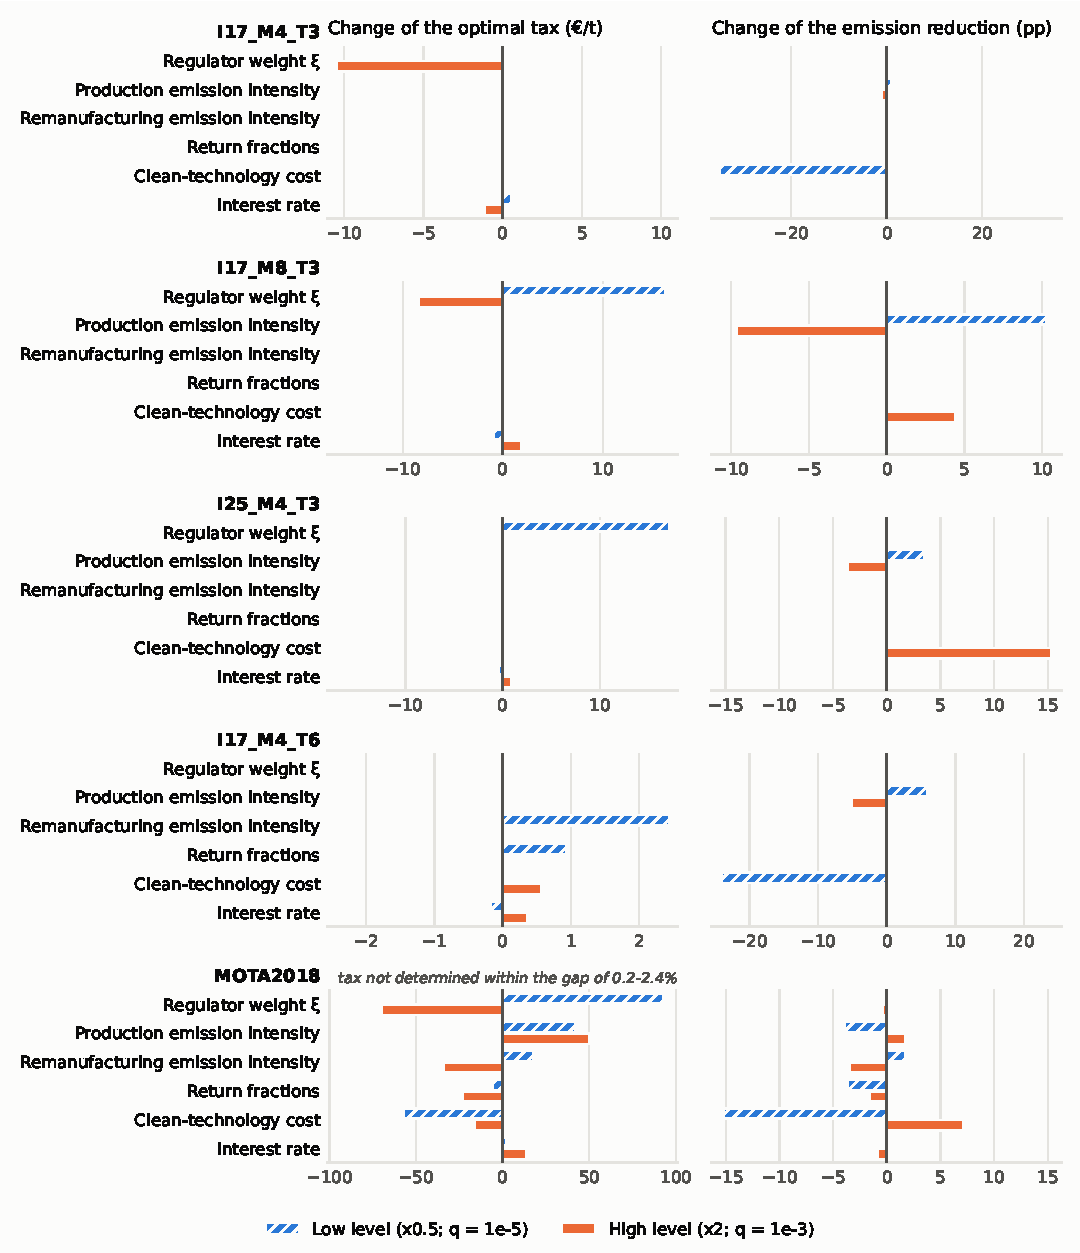
\includegraphics[width=\textwidth]{figures/sensitivity_tornado.pdf}
\caption{Change of the optimal tax (left, \EUR/t) and of the emission reduction (right, percentage points) from the base case when one parameter is set to its low level (blue, hatched) or its high level (orange); for the regulator's weight the levels are $\xi = 10^{-5}$ and $10^{-3}$. Rows: the four small instances and the case study; scales differ between rows. The case study's tax changes are not determined: its runs end with gaps of 0.2--2.4\% (Section~\ref{sec:sens-case}).}\label{fig:tornado}
\end{figure}

\paragraph{On most generated instances, the tax acts mainly through the choice of suppliers} We compare each network without a tax with the network at $\tau^*$ on the eleven closed instances. On nine of them, raw-material emissions fall by 2.7 to 97.3~kt \CO\ and account for 55--100\% of the reduction. On the other two, \inst{STD_I25_M4_T6} and \inst{STD_I25_M8_T12}, a change of production technology accounts for 86\% and 85\% of it. On the four small instances, the production technology changes on two (\inst{STD_I17_M4_T3} and \inst{STD_I17_M4_T6}) and the factory opened on two (\inst{STD_I17_M4_T3} and \inst{STD_I25_M4_T3}). Every network computed at \EUR0 and at \EUR74/t ships by truck only: transport makes up 0.1--0.6\% of the emissions, and the tax induces no modal shift. This agrees with \textcite{waltho2019green}, who find that carbon policies cut emissions mostly by moving the supply chain to lower-emitting resources, and with \textcite{palak2014analyzing}, where carbon regulation changes supplier selection. The case study behaves differently (Section~\ref{sec:sens-case}).

\paragraph{The optimal tax is set by the regulator's weight more than by the data} Lowering $\xi$ to $10^{-5}$ raises $\tau^*$ from \EUR16.5 to \EUR32.8/t on \inst{STD_I17_M8_T3} and from \EUR57.5 to \EUR74.6/t on \inst{STD_I25_M4_T3}. Raising $\xi$ to $10^{-3}$ lowers $\tau^*$ to \EUR8.0/t on \inst{STD_I17_M8_T3} and to \EUR23.4/t on \inst{STD_I17_M4_T3}. In every case the emission reduction changes by at most 0.23 percentage points: a regulator who weighs the tax level less buys the next break point, which abates almost nothing more. The interest rate moves $\tau^*$ by \EUR0.2 to \EUR1.9/t, and the other four parameters by at most \EUR2.4/t (on \inst{STD_I17_M4_T6}).

\paragraph{How much is abated depends on the cost of clean technology and on the production intensity} Halving the cost of the cleanest technology lowers the reduction from 52.5\% to 17.6\% on \inst{STD_I17_M4_T3} and from 44.1\% to 20.0\% on \inst{STD_I17_M4_T6}. The tax does not do less: the operator adopts the clean technology without a tax, so the network without a tax is already cleaner. Doubling that cost raises the reduction on \inst{STD_I25_M4_T3} from 11.7\% to 27.1\%; where the reduction stays the same, it raises the operator's cost increase, from 9.9\% to 15.6\% on \inst{STD_I17_M4_T3}. Halving and doubling the production intensity moves the reduction on \inst{STD_I17_M8_T3} from 27.2\% to 37.4\% and to 17.5\%, with the same $\tau^*$. The technologies installed at $\tau^*$ are the same in all 12 variants of each instance. \textcite{dong2025technology} reach a related conclusion under cap-and-trade: stricter regulation induces clean technology only if its efficiency exceeds a threshold.

\paragraph{Remanufacturing plays no role in the generated instances} Its share of production is at most 0.6\% in every variant, because remanufacturing emits about as much as production there (Section~\ref{sec:instances}). Its emission intensity and the return fractions change the reduction by at most 0.03 percentage points, and the return fractions only scale the share, from 0.29\% to 0.14\% and 0.58\% on \inst{STD_I17_M4_T3}. The case study, where remanufacturing is 16\% of production at the incumbent, is the test of these two parameters.

\subsection{Sensitivity analysis on the case study}\label{sec:sens-case}

On the case study the tax works through cleaner production technology and remanufacturing, and the cost of clean technology again has the largest effect on the reduction, which ranges from 8.2\% to 30.5\% (Table~\ref{tab:case}). No run closes its gap within 1~h; the gaps are 0.2--2.4\%. The case study has no raw-material emissions, and production makes up 94\% of its emissions at the base-case incumbent. Without a tax, the operator installs the higher-emission technology for one of its two products at both factories. At the incumbent it installs the lower-emission alternative for both products and remanufactures 16.0\% of production, against 4.2\% without a tax.

\begin{table}[!htbp]
\centering
\caption{Case study: response at the incumbent of each 1~h run, and bounds on the reduction at the optimum. The reduction and the cost increase are measured against each scenario's own network without a tax. The bounds follow from $\mathrm{LB} \le E^* + \mu\,\tau^* \le \mathrm{UB}$ with $\tau^* \in [0, 200]$~\EUR/t and $E^* \ge \Eref$, which give $E^* \in [\max(\Eref, \mathrm{LB} - 200\,\mu), \mathrm{UB}]$.}\label{tab:case}
\small
\begin{tabularx}{\textwidth}{@{}>{\raggedright\arraybackslash}p{4.6cm}*{5}{>{\raggedleft\arraybackslash}X}@{}}
\toprule
Scenario & Reduction at the incumbent (\%) & Reduction at the optimum, bounds (\%) & Operator's cost increase (\%) & Remanu\-facturing share (\%) & Gap (\%) \\
\midrule
Base & 23.4 & 22.6--25.0 & 1.4 & 16.0 & 1.2 \\
$\xi = 10^{-5}$ & 23.5 & 23.3--23.6 & 1.4 & 16.1 & 0.2 \\
$\xi = 10^{-3}$ & 23.0 & 20.3--25.9 & 1.1 & 15.5 & 2.4 \\
Production emission intensity $\times 0.5$ & 19.5 & 18.3--21.1 & 0.9 & 13.2 & 1.4 \\
Production emission intensity $\times 2$ & 25.2 & 24.1--26.6 & 1.4 & 16.1 & 1.5 \\
Remanufacturing emission intensity $\times 0.5$ & 25.2 & 24.3--26.9 & 1.4 & 16.1 & 1.6 \\
Remanufacturing emission intensity $\times 2$ & 19.9 & 19.4--21.6 & 1.1 & 14.5 & 1.2 \\
Return fractions $\times 0.5$ & 19.8 & 19.0--21.1 & 0.2 & 8.0 & 1.1 \\
Return fractions $\times 2$ & 21.9 & 21.2--23.9 & 1.3 & 16.8 & 1.4 \\
Clean-technology cost $\times 0.5$ & 8.2 & 7.8--11.1 & 1.2 & 15.8 & 1.6 \\
Clean-technology cost $\times 2$ & 30.5 & 29.9--32.3 & 2.1 & 16.0 & 1.5 \\
Interest rate 5\% & 23.3 & 22.5--24.8 & 1.3 & 16.1 & 1.0 \\
Interest rate 20\% & 22.6 & 21.7--24.8 & 1.5 & 16.0 & 2.1 \\
\bottomrule
\end{tabularx}
\end{table}

\paragraph{The optimal tax of the case study is not determined by these runs} The weight is $\mu = 3.08\cdot10^{6}$~kg per \EUR/t, so the base case's gap of 1.2\% leaves the tax open by about \EUR125/t; the incumbents' taxes are therefore not reported. The emissions are better determined. The reduction at the optimum lies within the bounds of Table~\ref{tab:case}, and the 3~h run of the base case reproduces its emissions within 0.07\% (Section~\ref{sec:robustness}). Five scenarios have bounds disjoint from those of the base case, so their change in the reduction is conclusive: the halved production intensity, the doubled remanufacturing intensity, the halved return fractions and both levels of the clean-technology cost. The bounds of the other scenarios overlap those of the base case, and their differences are inconclusive.

\paragraph{The network is robust} In every scenario the operator opens the same two factories and installs the same production technologies, the lower-emission alternative for each of the two products. The scenarios change volumes and the remanufacturing share, not the factories or the production technologies. The share responds to the return fractions asymmetrically because the case study already lets every unit sold return (a maximum return fraction of 1). Halving the fractions halves that ceiling and the share, from 16.0\% to 8.0\%. Doubling them leaves the ceiling at 1 and only doubles the minimum return, from 15\% to 30\% of sales, which raises the share to 16.8\%. Neither returns nor capacity bind: in the base case the operator collects 78\% of what could return and uses at most 47\% of the remanufacturing capacity in any period, so the volume remanufactured is an economic choice. That remanufacturing responds to the tax only where it carries an environmental advantage is consistent with \textcite{yenipazarli2016managing}, who characterises the taxes under which remanufacturing lowers emissions, and with \textcite{li2024optimal}, who find that a carbon tax does not always encourage remanufacturing.

\subsection{Robustness}\label{sec:robustness}

The sensitivity results on the small instances do not depend on the solver's tolerance. Re-solved at a MIP gap of $10^{-6}$ instead of $10^{-4}$, 51 of the 52 runs return the same optimal tax, to within \EUR0.05/t, and the same reduction, to within 0.1 percentage points. The 52 runs are the four base cases and the 48 variants of Section~\ref{sec:sens-small}; each took 8 to 178~s.

The exception is \inst{STD_I17_M8_T3} with twice the production intensity. At the tighter tolerance the run stalls after 15 iterations with its incumbent at \EUR8.77/t, against an optimal \EUR16.48/t at $10^{-4}$. Its lower bound is unchanged (259,574,947 against 259,574,944~kg), and the reduction differs by 0.1 points (17.4\% against 17.5\%). The optimum lies at a break point, where the operator is indifferent between two networks and the optimistic tie-break decides; which response it selects there depends on the follower's tolerance. This is the tax resolution of Proposition~\ref{prop:certificate} at work: the regulator's emissions are determined, the tax at the break point less so.

The results on the small instances do not depend on the solver's seed either. With seeds 0 to 4, 19 of the 20 runs on the four small instances return the same optimal tax, to within \EUR0.00001/t, the same reduction, the same result class and the same number of iterations; each run took 15 to 48~s. The exception is \inst{STD_I17_M4_T6} with seed 3, which ends $\varepsilon$-optimal after 4 iterations at \EUR7.55/t instead of \EUR7.17/t, with the same reduction. The two taxes lie on the same plateau, \EUR0.39/t apart, within the resolution of Proposition~\ref{prop:certificate}.

Giving the case study 3~h instead of 1~h narrows its gap from 1.2\% to 0.8\% over 10 iterations instead of 3. The incumbent's tax moves by \EUR36/t, while its emissions change by 0.07\% (31.873 against 31.894~Mt \CO) and the operator's cost by 0.05\%. This confirms Section~\ref{sec:sens-case}: on the case study the method determines the emissions and the network, but not the tax that induces them.

% =====================================================================================
\section{Conclusions}\label{sec:conclusions}

A regulator who anticipates how an operator redesigns its closed-loop supply chain can set the lowest tax that induces the operator's cleanest attainable network. We modelled this as a bilevel problem in which the regulator sets one carbon tax and the operator solves the network design model of \textcite{mota2018sustainable}. We showed that an optimal tax exists at a break point of the operator's value function, and solved the problem with the DBP of \textcite{soares2021deterministic}, adapted to a bilinear high-point relaxation. Within 1~h the method closes the gap to 0.01\% on 11 of 16 instances, with a certificate stated at the solver's tolerances (Proposition~\ref{prop:certificate}). On the other five it returns bounds, certified on all but two.

Four findings matter for policy, each on the instances named.
\begin{enumerate}
\item The optimal tax lies at a break point, the tax at which the operator switches to a cleaner network. Below it the network does not change; above it the operator pays more tax for further abatement that the regulator values at less than the extra tax, and that is small on every instance studied. A fixed tax at the 2025 EU allowance price achieves the same reduction on the nine closed instances whose break point lies below it, with a bill up to 73 times larger, but falls far short on the two whose break point lies above it.
\item The mechanism depends on where the emissions arise: lower-emission suppliers on nine of the eleven closed generated instances, a cleaner production technology on the other two, and cleaner technology with more remanufacturing on the case study, where production dominates. The transport mode never changed on the generated instances, where transport is under 0.6\% of emissions.
\item How much is abated depends more on the cost of clean technology than on the tax. When the clean technology is cheap, the operator adopts it without a tax, and the tax has little left to do.
\item The optimal tax is set by the regulator's trade-off between emissions and the tax level more than by the data: $\xi$ moves it far more than any of the five data parameters, while barely changing the abatement.
\end{enumerate}

The study has limits that point to further work. On the method: with one tax, enumerating break points is an exact alternative (Section~\ref{sec:enumeration}), and a computational comparison would also verify the taxes reported here. The HPR dominates the computing time, and discretisation schemes such as multiparametric disaggregation \parencite{kolodziej2013global} could tighten it. The certificate fixes the tax only to about \EUR1/t on a plateau, and the case study's tax not at all within 1--3~h. On the model: the tax is a single rate. A tax per emission source or per period, such as the differential taxes compared by \textcite{xia2025comparative}, makes the leader's decision a vector; the DBP applies in principle, with one bilinear term per tax in the HPR, but enumeration no longer does. The regulator does not maximise welfare \parencite{krass2013environmental,rustico2022environmental}, and the operator does not compete; under competition, emissions may even rise with the tax \parencite{krass2025competitive}. The model is deterministic, while demand, returns and the price of carbon are uncertain \parencite{haddadsisakht2018closed,beck2023survey}. On the data: the generated instances' emission factors are large relative to costs and give remanufacturing no advantage; a recalibrated generator would let them speak to the closed-loop findings too.

% =====================================================================================
% =====================================================================================
%% Declarations required by the EJOR Guide for Authors (single-anonymized review: they stay in the manuscript).
\section*{CRediT authorship contribution statement}
%% TODO(author): adapt to the actual contributions of every author.
\textbf{Marcelo Pinto:} Conceptualization, Methodology, Software, Investigation, Formal analysis, Data curation, Visualization, Writing -- original draft. \textbf{TODO Co-author:} Supervision, Writing -- review \& editing.

\section*{Declaration of competing interest}
%% TODO(author): confirm.
Declarations of interest: none.

\section*{Funding}
%% TODO(author): FCT grant reference, or the sentence below if there is no specific funding.
This work was supported by Funda\c{c}\~{a}o para a Ci\^{e}ncia e a Tecnologia (FCT) [grant number TODO]. The funding source had no role in the study design; in the collection, analysis and interpretation of data; in the writing of the report; or in the decision to submit the article for publication.

\section*{Data availability}
%% TODO(author): repository URL and archived DOI.
The code, the instances and the raw results of every run are available at TODO (archived at TODO DOI).

\section*{Declaration of generative AI and AI-assisted technologies in the writing process}
%% TODO(author): describe the actual use. Statement wording from the EJOR Guide for Authors.
During the preparation of this work the author(s) used Claude (Anthropic) in order to TODO describe the use, for example revise the language and structure of the text and check the references against the publishers' records. After using this tool, the author(s) reviewed and edited the content as needed and take(s) full responsibility for the content of the publication.

\printbibliography

\end{document}
